% Whitepaper: jena-intrinsic-provenance
% Build with scripts/build-whitepaper.sh (latexmk + pdflatex + biber).

\documentclass[11pt,a4paper]{article}

% ---------------------------------------------------------------- Fonts and layout
\usepackage[T1]{fontenc}
\usepackage[utf8]{inputenc}
\usepackage{amsmath}
\usepackage{libertinus}
\usepackage[varqu,varl,scaled=0.95]{inconsolata}
\usepackage[a4paper,left=28mm,right=28mm,top=26mm,bottom=30mm]{geometry}
\usepackage{microtype}
\usepackage{xcolor}
\usepackage{titlesec}
\usepackage{fancyhdr}
\usepackage[font=small,labelfont={bf,sf},labelsep=period]{caption}
\usepackage{booktabs}
\usepackage{tabularx}
\usepackage{array}
\usepackage{enumitem}
\usepackage{listings}
\usepackage{needspace}
\usepackage{placeins}
\usepackage{tikz}
\usetikzlibrary{arrows.meta,positioning,fit,calc,shapes.geometric,shapes.symbols,decorations.pathreplacing}
\usepackage[backend=biber,style=numeric,sorting=none,maxbibnames=4,giveninits=true,
            doi=false,isbn=false,eprint=false,urldate=iso]{biblatex}
\usepackage{csquotes}
\usepackage{xurl}
\usepackage{hyperref}

\addbibresource{references.bib}
% Keep ISO access dates (2026-11-15) on one line; biblatex's default plus \mbox.
\DeclareFieldFormat{urldate}{\mkbibparens{\bibstring{urlseen}\space\mbox{#1}}}

\definecolor{accent}{RGB}{0,84,147}
\definecolor{codebg}{RGB}{246,246,244}
\definecolor{kw}{RGB}{0,70,140}
\definecolor{str}{RGB}{120,60,0}
\definecolor{cmt}{RGB}{100,100,100}
\definecolor{brk}{gray}{0.6}
\definecolor{provEntity}{HTML}{FFFC87}
\definecolor{provActivity}{HTML}{9FB1FC}
\definecolor{provAgent}{HTML}{FED37F}

\hypersetup{
  colorlinks=true, linkcolor=accent, citecolor=accent, urlcolor=accent, bookmarksdepth=2,
  pdftitle={Provenance for Apache Jena},
  pdfauthor={Lars Wilhelmsen <lars@sral.org>},
  pdfsubject={A persistent data version for TDB2 and signed attestations for SPARQL results},
  pdfkeywords={Apache Jena, TDB2, Fuseki, SPARQL, provenance, PROV-O, RDFC-1.0, Data Integrity, ecdsa-rdfc-2019, PKCS\#11, RFC 3161},
}
\urlstyle{same}

\setlength{\parskip}{0.45em}
\setlength{\parindent}{0pt}
\linespread{1.06}

\titleformat{\section}{\sffamily\Large\bfseries\color{accent}}{\thesection}{0.7em}{}
\titleformat{\subsection}{\sffamily\large\bfseries}{\thesubsection}{0.7em}{}
\titleformat{\subsubsection}{\sffamily\normalsize\bfseries}{\thesubsubsection}{0.7em}{}
\titlespacing*{\section}{0pt}{1.6em}{0.6em}
\titlespacing*{\subsection}{0pt}{1.2em}{0.4em}

\pagestyle{fancy}
\fancyhf{}
\fancyhead[L]{\sffamily\small\color{black!60}Provenance for Apache Jena}
\fancyhead[R]{\sffamily\small\color{black!60}\thepage}
\renewcommand{\headrulewidth}{0pt}
\fancypagestyle{plain}{\fancyhf{}\fancyfoot[C]{\sffamily\small\color{black!60}\thepage}}

\setlist{itemsep=0.15em, topsep=0.3em}

% Inline conventions (O'Reilly style): constant width for code and IRIs, italic for files.
\newcommand{\code}[1]{\texttt{#1}}
\newcommand{\file}[1]{\textit{#1}}
% Long identifiers that may break at any character, like URLs.
\DeclareUrlCommand\longcode{\urlstyle{tt}}
\renewcommand{\arraystretch}{1.25}
% Replaceable parts inside code (Inconsolata has no italic).
\newcommand{\repl}[1]{\textrm{\textit{#1}}}
\setlength{\emergencystretch}{2em}

% ---------------------------------------------------------------- Listings
\renewcommand{\lstlistingname}{Example}
\lstdefinestyle{base}{
  basicstyle=\ttfamily\small,
  columns=fullflexible, keepspaces=true, upquote=true,
  showstringspaces=false, breaklines=true,
  postbreak=\mbox{\textcolor{brk}{$\hookrightarrow$}\space},
  backgroundcolor=\color{codebg}, frame=single, rulecolor=\color{codebg},
  framesep=5pt, xleftmargin=5pt, xrightmargin=5pt,
  aboveskip=0.9em, belowskip=0.6em, captionpos=t,
  keywordstyle=\color{kw}\bfseries, stringstyle=\color{str},
  commentstyle=\color{cmt},
}
\lstdefinelanguage{SPARQL}{
  sensitive=true,
  morekeywords={PREFIX,SELECT,WHERE,SERVICE,SILENT,OPTIONAL,ORDER,BY,GRAPH,INSERT,DATA,AS,LIMIT},
  morecomment=[l]{\#},
  morestring=[s]{<}{>},
  morestring=[b]",
}
\lstdefinelanguage{Turtle}{
  sensitive=true,
  morekeywords={PREFIX,a,true,false},
  morecomment=[l]{\#},
  morestring=[s]{<}{>},
  morestring=[b]",
}
\lstset{style=base}

% ---------------------------------------------------------------- Title
\title{\sffamily\bfseries\color{accent}Provenance for Apache Jena\\[0.4em]
  \Large\mdseries\color{black}A Persistent Data Version for TDB2 and\\Signed Attestations for SPARQL Results}
\author{\large Lars Wilhelmsen\\[0.2em]\normalsize\href{mailto:lars@sral.org}{\texttt{lars@sral.org}}}
\date{\normalsize Proof-of-concept report, jena-intrinsic-provenance 0.17.0-SNAPSHOT\\[0.2em]November 2026}

\begin{document}

\maketitle
\thispagestyle{plain}

\begin{abstract}
\noindent
A SPARQL endpoint answers a query with a table of solutions but says nothing about where the
solutions came from. A client cannot tell which state of the database produced the answer, and
anyone who receives the table later cannot check that it is what the server sent. This report
describes a proof of concept for Apache Jena and its Fuseki SPARQL server, version 6.2.0, that
closes both gaps. The first part is a persistent data version for TDB2, Jena's transactional
storage engine: a counter that increases by one with every committed write transaction. The
counter is written to TDB2's journal in the same commit as the data, so restarts, compaction,
and crashes leave it consistent with the data. The second part is
a SPARQL \code{SERVICE} that attests the solutions of the pattern inside it. Each result
attestation is a PROV-O graph that names the database state and the authenticated user who
asked for it. It records a SHA-256 digest of the solutions after RDF Dataset Canonicalization
(RDFC-1.0) and carries a W3C Data Integrity proof. By default, the proof is made with the
\code{ecdsa-rdfc-2019} cryptosuite by a P-256 or P-384 key that never leaves a PKCS\#11 token in
a separate signer process. An Ed25519 key file with \code{eddsa-rdfc-2022} is an alternative.
An RFC~3161 time-stamping authority can additionally co-sign the attestation in the
background, which establishes when the attestation existed independently of the server's clock
and without delaying the query. A standalone verifier checks a saved result against its
attestation without contacting the server. The implementation passes all 65 tests of the W3C
RDFC-1.0 test suite and agrees with the \code{eddsa-rdfc-2022} and \code{ecdsa-rdfc-2019} test
vectors. It digests 10,000 solutions, the default maximum, in less than 0.4~s.
\end{abstract}
\clearpage

\setcounter{tocdepth}{1}
\tableofcontents
\clearpage

% ====================================================================================
\section{Introduction}
\label{sec:intro}

SPARQL results often outlive the request that produced them. They end up in reports, caches,
and data pipelines, and they reach people who never talked to the endpoint. Whoever holds such
a result later has two questions that the result cannot answer by itself: which state of the
data it was computed from, and whether it is still exactly what the server returned.

This report describes a proof of concept that answers both questions for Apache
Jena~\cite{jena} and its Fuseki server, version 6.2.0. The work started from two research
questions:

\begin{enumerate}[label=\textbf{RQ\arabic*}, leftmargin=3em]
\item Can TDB2, Jena's transactional storage engine, expose a unique, monotonically increasing
  value that changes on every write transaction?
\item Can a query that refers to a specially named \code{SERVICE} receive a provenance
  attestation, based on PROV-O~\cite{provo}, that binds its result with RDF Dataset
  Canonicalization (RDFC-1.0)~\cite{rdfc} and is digitally signed?
\end{enumerate}

% ###AQ: The route through the report covers Sections 3-7 only; mention Section 2 and the appendices?
TDB2 already keeps a counter of the kind RQ1 asks for, but only in memory, so it starts from
zero every time the database is opened. Section~\ref{sec:version} describes a persistent
counter that TDB2 writes to its own journal in the same commit as the data, and the assembler
that recovers it after a crash. For RQ2, Section~\ref{sec:cert} describes a \code{SERVICE}
that evaluates the pattern inside it, encodes the solutions as RDF, and canonicalizes and
hashes them. It signs a PROV-O attestation with the W3C Data Integrity cryptosuite
\code{ecdsa-rdfc-2019}~\cite{vcdi,ecdsa}, using a key held on a PKCS\#11 token in a separate
process. The same section covers the recording of the authenticated user, optional
timestamps from an RFC~3161 time-stamping authority, and the offline verifier.
Section~\ref{sec:fuseki} shows how the module plugs into Fuseki without changes to Jena,
Section~\ref{sec:eval} reports tests and measurements, and Section~\ref{sec:discussion}
discusses what an attestation proves and what it leaves open.

Figure~\ref{fig:architecture} shows the parts of the system and the path of an attested query.
The client sends an ordinary SPARQL query to Fuseki. The attest executor evaluates the inner
pattern in a read transaction on the versioned dataset, stores a signed attestation in a
separate database, and returns the rows with the attestation IRI attached. The client can then
fetch the attestation and verify the rows offline.

\begin{figure}[htbp]
\centering
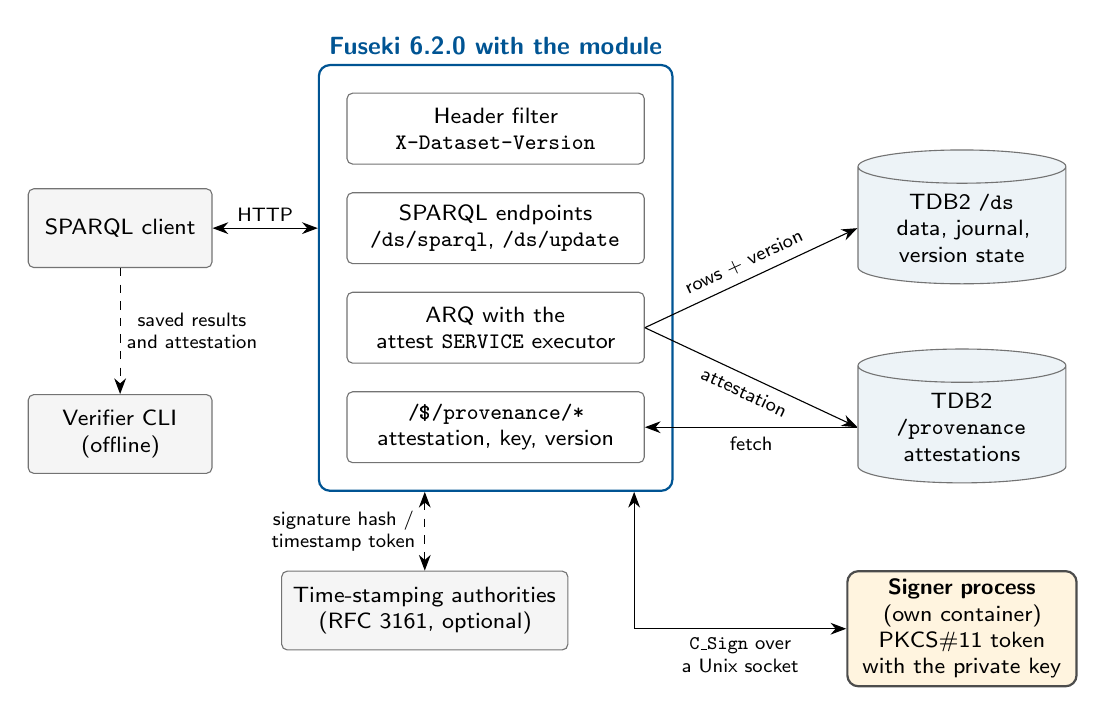
\begin{tikzpicture}[
  font=\sffamily\footnotesize,
  >={Stealth[length=2mm]},
  comp/.style={draw=black!55, fill=white, rounded corners=2pt, align=center,
               minimum height=9mm, text width=36mm, inner sep=2.5pt},
  store/.style={cylinder, shape border rotate=90, aspect=0.16, draw=black!55,
                fill=accent!7, align=center, text width=25mm, minimum height=17mm, inner sep=2pt},
  ext/.style={draw=black!55, fill=black!4, rounded corners=2pt, align=center,
              text width=21mm, minimum height=10mm},
  lbl/.style={font=\sffamily\scriptsize, fill=white, inner sep=1.2pt, align=center},
]
\node[comp] (filter) {Header filter\\\texttt{X-Dataset-Version}};
\node[comp, below=3.5mm of filter] (sparql) {SPARQL endpoints\\\texttt{/ds/sparql}, \texttt{/ds/update}};
\node[comp, below=3.5mm of sparql] (arq) {ARQ with the\\attest \texttt{SERVICE} executor};
\node[comp, below=3.5mm of arq] (servlet) {\texttt{/\$/provenance/*}\\attestation, key, version};
\node[draw=accent, thick, rounded corners=4pt, fit=(filter)(servlet), inner sep=3.5mm] (fuseki) {};
\node[font=\sffamily\small\bfseries, text=accent, anchor=south] at (fuseki.north) {Fuseki 6.2.0 with the module};

\node[ext, left=17mm of sparql] (client) {SPARQL client};
\node[ext, below=16mm of client] (verify) {Verifier CLI\\(offline)};

\node[store, right=27mm of sparql] (ds) {TDB2 \texttt{/ds}\\data, journal,\\version state};
\node[store, right=27mm of servlet] (prov) {TDB2\\\texttt{/provenance}\\attestations};

\draw[<->] (client.east) -- node[lbl, above=1pt] {HTTP} (fuseki.west |- client.east);
\draw[->, dashed] (client.south) -- node[lbl, right=1pt] {saved results\\and attestation} (verify.north);
\draw[->] (arq.east) -- node[lbl, above=2pt, sloped, pos=0.5] {rows + version} (ds.west);
\draw[->] (arq.east) -- node[lbl, below=2pt, sloped, pos=0.5] {attestation} (prov.west);
\draw[<-] (servlet.east) -- node[lbl, below=2pt] {fetch} (prov.west);

\node[ext, text width=34mm, anchor=north] (tsa) at ($(fuseki.south) + (-9mm,-10mm)$) {Time-stamping authorities\\(RFC 3161, optional)};
\draw[<->, dashed] ($(fuseki.south) + (-9mm,0)$) -- node[lbl, left=2pt] {signature hash /\\timestamp token} (tsa.north);
\node[draw=black!70, thick, fill=provAgent!25, rounded corners=4pt, align=center, text width=27mm,
      inner sep=3pt, below=11mm of prov] (signer) {\textbf{Signer process}\\(own container)\\PKCS\#11 token\\with the private key};
\draw[<->] ($(fuseki.south east) + (-5mm,0)$) |- node[lbl, pos=0.75, below=2pt] {\texttt{C\_Sign} over\\a Unix socket} (signer.west);
\end{tikzpicture}
\caption{Components of the proof of concept and the path of an attested query. The signing key
stays in a separate signer process (Figure~\ref{fig:separation}); Fuseki asks it for each
signature. If time-stamping authorities are configured, a background worker asks one of them
to co-sign each attestation after the query has returned.}
\label{fig:architecture}
\end{figure}

The module runs on Java 21 and is loaded into the unmodified Fuseki server. The verifier is
a separate library that needs neither TDB2 nor Fuseki (Section~\ref{sec:verification}). The
module's vocabulary uses the namespace \code{jip:} (\code{https://larsw.xyz/jip/}) and is
defined in \file{vocab/jip.ttl}. The Maven group ID is \code{xyz.larsw}, and the Java
packages are under \code{xyz.larsw.jip}.

\subsection*{Conventions}

Constant width marks code, IRIs, SPARQL, and configuration terms. Italic marks file names and
terms at the point where they are defined. The signed statements the module produces are called
\emph{result attestations}, and a query that asks for one is an \emph{attested query}. The word
\emph{certificate} is reserved for X.509 certificates, such as the one a time-stamping
authority signs with. Table~\ref{tab:prefixes} lists the namespace prefixes used in the
examples.

\begin{table}[htbp]
\centering
\caption{Namespace prefixes used in this report.}
\label{tab:prefixes}
\small
\begin{tabular}{@{}ll@{}}
\toprule
Prefix & Namespace IRI \\
\midrule
\code{jip:} & \code{https://larsw.xyz/jip/} (this module's vocabulary, Appendix~\ref{app:vocab}) \\
\code{prov:} & \code{http://www.w3.org/ns/prov\#} \\
\code{sec:} & \code{https://w3id.org/security\#} \\
\code{dcterms:} & \code{http://purl.org/dc/terms/} \\
\code{rs:} & \code{http://www.w3.org/2001/sw/DataAccess/tests/result-set\#} \\
\code{xsd:} & \code{http://www.w3.org/2001/XMLSchema\#} \\
\code{tdb2:} & \code{http://jena.apache.org/2016/tdb\#} \\
\code{ja:} & \code{http://jena.hpl.hp.com/2005/11/Assembler\#} \\
\code{sd:} & \code{http://www.w3.org/ns/sparql-service-description\#} \\
\code{ex:} & \code{http://example.org/} \\
\bottomrule
\end{tabular}
\end{table}

% ====================================================================================
\section{Background}
\label{sec:background}
% ###AQ: Add a lead-in sentence saying what Section 2 covers (standards, then related approaches)?

\subsection{Transactions in TDB2}
\label{sec:tdb-txn}

TDB2 stores an RDF dataset on disk and gives it ACID transactions with multiple concurrent
readers and a single writer. The transaction machinery lives in a lower layer called DBOE
(Database Operating Environment). There, a \emph{transaction coordinator} drives a set of \emph{transactional components}: the
node table, the indexes, the prefix table, and anything else registered with it. Each component
has an ID and takes part in every transaction through callbacks such as \code{\_begin},
\code{\_commitPrepare}, \code{\_commit}, and \code{\_commitEnd}.

A write transaction commits in five steps, all driven by \code{TransactionCoordinator}:

\begin{enumerate}
\item \emph{Prepare}. Each component may return a REDO record, which the coordinator appends
  to the journal file, \file{Data-0001/journal.jrnl}.
\item \emph{Commit point}. The coordinator appends a COMMIT entry and forces the journal to
  disk. From here on the transaction is durable.
\item \emph{Commit}. Each component makes its changes permanent.
\item The coordinator truncates the journal.
\item \emph{Commit end}. The components make the new state visible to later transactions, and
  the coordinator increments its data version counter (Section~\ref{sec:tdb-has}).
\end{enumerate}

Steps 2--5 run while the coordinator holds its lock. Transactions begin under the same lock,
so a new transaction sees either the state before the commit or the state after it.

When a database opens, the coordinator reads the journal. For every transaction that has a
COMMIT entry, it passes each REDO record to the component with the matching ID. If no component
with that ID is registered, it logs \code{No component for ...} and skips the record. That
detail shapes the design in Section~\ref{sec:recovery}.

\subsection{RDF Dataset Canonicalization}
\label{sec:rdfc}

Hashing RDF is harder than hashing a file because one dataset has many serializations.
Statement order can vary, and blank nodes have no global names, so two serializations of the
same dataset can use different blank node labels. RDFC-1.0~\cite{rdfc} gives every blank node
a canonical label (\code{c14n0}, \code{c14n1}, and so on) derived from its surroundings, and
serializes the dataset as sorted N-Quads. Isomorphic datasets produce identical canonical
N-Quads, so a hash of that text identifies the dataset independently of how it was written
down.

The algorithm first computes a \emph{first-degree hash} for each blank node from the quads
that mention it. A blank node whose first-degree hash is unique gets its label right away. The
others go through the \emph{N-degree hash} algorithm, which explores paths to neighboring blank
nodes. That step is exponential in the worst case. The specification discusses datasets built
to exploit this behavior under the name \emph{dataset poisoning}, so an implementation has to
limit the work it is willing to do. Section~\ref{sec:perf} shows how the encoding used here
interacts with the two steps.

\subsection{Data Integrity Proofs}
\label{sec:di}

The W3C specification Verifiable Credential Data Integrity~1.0~\cite{vcdi} describes how to attach
a proof to a document. A proof names a cryptosuite, a verification method (the key), a
purpose, and a creation time. The cryptosuite \code{eddsa-rdfc-2022}~\cite{eddsa} works on
the RDF form of the document. It canonicalizes the proof options and the document separately
with RDFC-1.0, hashes each with SHA-256, concatenates the two hashes, and signs the result with
Ed25519~\cite{rfc8032}. The signature is stored as a multibase string in base58btc encoding,
recognizable by its leading \code{z}.

The cryptosuite \code{ecdsa-rdfc-2019}~\cite{ecdsa} has the same structure but signs with
ECDSA on the NIST curves P-256 or P-384. The hash is SHA-256 for P-256 and SHA-384 for
P-384, and the signature is the concatenation $r \Vert s$ of its two integers.

The verification method used here is a \code{did:key}~\cite{didkey}, a decentralized identifier
(DID) that contains the public key. A verifier reads the key out of the identifier and
does not need to fetch anything. The key type is part of the identifier: Ed25519 keys start with
\code{z6Mk}, P-256 keys with \code{zDn}, and P-384 keys with \code{z82}.

\subsection{PKCS\#11}
\label{sec:pkcs11}

PKCS\#11~\cite{pkcs11} is the standard C interface to cryptographic tokens: hardware security
modules (HSMs), smart cards, cloud key services, and software tokens such as
SoftHSM2~\cite{softhsm}. An application loads the token's \emph{module}, which is a shared
library. It then logs in with a PIN, finds a key by its label, and asks the token to sign with it
(\code{C\_SignInit}, \code{C\_Sign}). A private key created on the token with the
non-extractable flag never leaves it; the application only ever holds a handle. Java reaches
PKCS\#11 through the JDK's SunPKCS11 provider.

A PKCS\#11 module normally runs inside the application's process. The p11-kit
tools~\cite{p11kit} separate the two. The command \code{p11-kit server} loads the real module
in one process and serves it on a Unix socket. The application loads \code{p11-kit-client.so}, a module that forwards every
PKCS\#11 call over that socket. To the application it is an ordinary token.

\subsection{Trusted Timestamps}
\label{sec:tsp}

A signature shows who signed something, but its creation time is whatever the signer wrote
into it. The Time-Stamp Protocol of RFC~3161~\cite{rfc3161} adds a second party. A client sends a
\emph{time-stamping authority} (TSA) the hash of some data, the \emph{message imprint}. The TSA
returns a \emph{time-stamp token}: a signed structure in the Cryptographic Message Syntax
(CMS) that contains the imprint, the
TSA's time (\code{genTime}), a serial number, and the nonce of the request. The TSA signs it
with a certificate whose extended key usage is \code{id-kp-timeStamping}. Anyone who has the data and
the token can check, offline, that the data existed no later than \code{genTime}, as far as they
trust the TSA. Code signing and long-term signature formats such as CMS Advanced Electronic
Signatures (CAdES) use the same construction to timestamp a signature value. Several public
TSAs answer such requests free of charge.

\subsection{PROV-O}
\label{sec:provo}

PROV-O~\cite{provo} is the W3C ontology for provenance. It describes \emph{entities}, such as
a dataset or a query result; \emph{activities}, such as a query execution; and \emph{agents},
which are responsible for activities, such as a server. The attestation in
Section~\ref{sec:attestation} uses the relations \code{prov:wasGeneratedBy}, \code{prov:used},
\code{prov:wasDerivedFrom}, \code{prov:wasAssociatedWith}, \code{prov:qualifiedAssociation}, and
\code{prov:specializationOf}, and the activity times \code{prov:startedAtTime} and
\code{prov:endedAtTime}.

\subsection{Related Approaches}
\label{sec:related}

The problem touches three lines of earlier work: keeping versions of RDF data, making
published RDF verifiable, and making database contents or query results checkable.

Several systems keep the history of an RDF dataset. R43ples~\cite{r43ples} stores the
differences between revisions of named graphs in additional graphs and serves the revisions
through SPARQL. The Quit Store~\cite{quitstore} versions RDF datasets in Git, with branches,
merges, and the provenance of each change. OSTRICH~\cite{ostrich} is a compressed triple store
that answers queries at any version of an RDF archive. Unlike the module described here
(Section~\ref{sec:reproduce}), these systems can query earlier states, but each is a separate
store or a layer in front of one. None gives an unmodified TDB2 a version that is committed
atomically with its data.

Signing RDF depends on a canonical form. Carroll~\cite{carroll2003} showed that signing
arbitrary RDF graphs is hard in general and proposed signatures for graphs that can be
canonicalized cheaply. RDFC-1.0 handles any dataset, within a work limit
(Section~\ref{sec:rdfc}). Trusty URIs~\cite{trustyuri} put a hash of the content into the URI,
so that an artifact such as a nanopublication can be verified and cannot change without
changing its name. Verifiable Credentials~\cite{vcdm2} carry claims about a subject and can be
secured with the Data Integrity proofs this module uses. All three secure documents that
someone publishes, not the answer an endpoint computes from its current data.

In databases, provenance often means how each result tuple was derived from the input tuples,
which provenance semirings~\cite{green2007} describe in general. An attestation instead records
which database state and which server produced a result. Authenticated data
structures~\cite{li2006} let a client verify that the answer to a range query is correct and
complete against a digest the data owner signed. That is a stronger guarantee than an
attestation gives, but it needs special index structures in the database. Ledger databases
such as SQL Ledger~\cite{sqlledger} keep tamper-evident digests of the data's history, so that
changes to stored data can be detected; they do not cover query results. This report combines
a data version and verifiable results for the stock Jena and Fuseki. The version is committed
atomically with the data, and signed attestations bind each SPARQL result to it.

% ====================================================================================
\section{A Persistent Data Version for TDB2}
\label{sec:version}
% ###AQ: Add a lead-in sentence saying what Section 3 covers?

\subsection{What TDB2 Already Has}
\label{sec:tdb-has}

Reading the 6.2.0 sources of \code{jena-dboe-transaction}, \code{jena-tdb2}, and
\code{jena-fuseki-main} produced the findings in Table~\ref{tab:findings}.

\begin{table}[ht]
\centering
\caption{What Jena 6.2.0 provides for versioning a TDB2 database.}
\label{tab:findings}
\small
\begin{tabularx}{\linewidth}{@{}>{\raggedright\arraybackslash}X>{\raggedright\arraybackslash}p{38mm}@{}}
\toprule
Finding & Where \\
\midrule
The coordinator keeps an \code{AtomicLong dataVersion}. \code{advanceDataVersion()} increments
it once per committed write transaction, inside the commit critical section. Reads and aborts
leave it alone. & \code{TransactionCoordinator} \\
Each transaction records the version it started from, and \code{getDataVersion()} is public.
& \code{Transaction} \\
The counter exists only in memory and starts at 0 when the coordinator is created. Compaction
copies it to the new coordinator. & \code{TransactionCoordinator}, \code{DatabaseOps.compact} \\
Nothing on disk changes exactly once per commit. The journal is truncated after every commit,
and the index files change only when the data change and are rewritten by compaction.
& \code{TransactionCoordinator}, \code{DatabaseOps} \\
A running coordinator accepts extra components through \code{modifyConfig} and
\code{addExternal}, which \code{jena-text} also uses. Compaction moves them to the new
coordinator. & \code{TransactionCoordinator}, \code{DatabaseOps.compact} \\
TDB2's own components use IDs 1 to 51. & \code{ComponentIdMgr} \\
Fuseki builds the datasets in its configuration file in \code{parseConfig}, before any
\code{FusekiModule} hook runs. & \code{FusekiServer} \\
\bottomrule
\end{tabularx}
\end{table}

The internal counter behaves correctly within one process, but it is not unique over time:
version 5 before a restart and version 5 after a restart can describe different data. The
module still exposes it, as the function \code{jip:tdbDataVersion()}, so the two counters can
be compared.

\subsection{Requirements}
\label{sec:requirements}

The persistent version has to meet six requirements:

\begin{enumerate}[label=\textbf{R\arabic*}, leftmargin=3em]
\item A pair of database ID and version identifies exactly one committed state, for the
  lifetime of the database.
\item Every committed write transaction increments the version by one. Reads and aborted
  writes do not change it.
\item After a crash, the version on disk matches the data on disk.
\item The version survives restarts and compaction.
\item A transaction sees the version that belongs to its data snapshot.
\item Jena itself stays unchanged, and the module works with the stock Fuseki 6.2.0 server.
\end{enumerate}

\subsection{An External Transactional Component}
\label{sec:component}

The persistent counter is a DBOE component, \code{DataVersionComponent}, added to the TDB2
coordinator with \code{addExternal}. Its ID is \code{0x50524F56}, the ASCII bytes of
\enquote{PROV}, well outside the range TDB2 uses for its own components.
Table~\ref{tab:lifecycle} shows what the component does in each callback, and
Example~\ref{lst:component} shows the commit path.

\begin{table}[ht]
\centering
\caption{What \code{DataVersionComponent} does during a transaction.}
\label{tab:lifecycle}
\small
\begin{tabularx}{\linewidth}{@{}>{\raggedright\arraybackslash}p{30mm}>{\raggedright\arraybackslash}X@{}}
\toprule
Callback & Action \\
\midrule
\code{\_begin} & Copies the committed version into the transaction state and records it for
the HTTP headers (Section~\ref{sec:exposure}). \\
\code{\_commitPrepare} & Write transactions only: computes $\mathit{next} =
\mathit{committed} + 1$ and returns the REDO record (format~1, $\mathit{next}$), which the
coordinator appends to the journal. \\
\textit{commit point} & The coordinator appends COMMIT and forces the journal to disk. \\
\code{\_commit} & Rewrites \file{jip-data-version.properties} in the database directory:
temporary file, \code{fsync}, atomic rename, \code{fsync} of the directory. \\
\code{\_commitEnd} & Publishes $\mathit{next}$ as the committed version and records it for the
headers. \\
\code{\_abort} & Persists nothing. \\
\bottomrule
\end{tabularx}
\end{table}

\Needspace{10\baselineskip}
\begin{lstlisting}[language=Java, caption={The commit path of \code{DataVersionComponent} (comments shortened).}, label={lst:component}]
@Override
protected ByteBuffer _commitPrepare(TxnId txnId, TxnVersion state) {
    if ( !isWriteTxn() )
        return null;
    // Single writer: committed cannot change between here and commitEnd.
    state.next = committed.get() + 1;
    return encodeRedo(state.next);           // int format, long version
}

@Override
protected void _commit(TxnId txnId, TxnVersion state) {
    if ( !isWriteTxn() )
        return;
    // After the journal commit point. If this fails, the journal entry is replayed.
    if ( stateFile != null )
        stateFile.write(new DataVersionStateFile.State(databaseId, state.next));
}

@Override
protected void _commitEnd(TxnId txnId, TxnVersion state) {
    if ( !isWriteTxn() )
        return;
    committed.set(state.next);
    RequestVersionTracker.observeCommit(this, state.next);
}
\end{lstlisting}

The component increments the version on every committed write transaction, including one that
changes nothing. This matches TDB2's internal counter, so within one process the difference
between the persistent and the internal version stays constant; a test checks this. It also
means that equal versions imply equal data, whereas different versions do not necessarily
mean different data.

\code{\_begin}, \code{\_commit}, and \code{\_commitEnd} run under the coordinator lock.
\code{\_commitPrepare} runs outside it, but TDB2 allows only one writer at a time, so the
committed version cannot change between prepare and commit end. A transaction therefore sees
the version that belongs to its snapshot (R5). The test
\code{readersSeeTheirSnapshotVersion} checks this with readers that hold their transactions
open while a writer commits.

\subsection{Recovery Before the Database Opens}
\label{sec:recovery}

A process can crash at any point of the commit sequence. Figure~\ref{fig:crash} marks the
three cases that matter for the version.

\begin{figure}[ht]
\centering
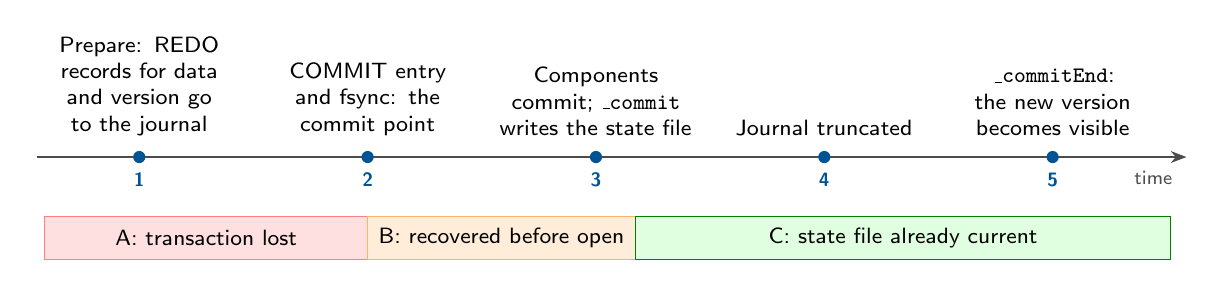
\begin{tikzpicture}[font=\sffamily\footnotesize, >={Stealth[length=2mm]}]
\draw[->, thick, black!70] (0,0) -- (14.6,0) node[below left=2pt, font=\sffamily\scriptsize] {time};
\foreach \x/\n/\t in {
    1.3/1/{Prepare: REDO records for data and version go to the journal},
    4.2/2/{COMMIT entry and fsync: the commit point},
    7.1/3/{Components commit; \texttt{\_commit} writes the state file},
    10.0/4/{Journal truncated},
    12.9/5/{\texttt{\_commitEnd}: the new version becomes visible}} {
  \fill[accent] (\x,0) circle (2.2pt);
  \node[above, align=center, text width=26mm] at (\x,0.15) {\t};
  \node[below, font=\sffamily\scriptsize\bfseries, text=accent] at (\x,-0.08) {\n};
}
\draw[fill=red!12, draw=red!50] (0.1,-0.75) rectangle node {A: transaction lost} (4.2,-1.3);
\draw[fill=orange!15, draw=orange!60] (4.2,-0.75) rectangle node {B: recovered before open} (7.6,-1.3);
\draw[fill=green!12, draw=green!50!black] (7.6,-0.75) rectangle node {C: state file already current} (14.4,-1.3);
\end{tikzpicture}
\caption{Commit sequence of a write transaction and the three crash windows for the version.}
\label{fig:crash}
\end{figure}

\begin{description}[font=\normalfont\itshape, leftmargin=1.5em, style=nextline]
\item[Crash in window A.] The journal has no COMMIT entry for the transaction, so TDB2
  discards it on restart. Data and version both stay at the previous state.
\item[Crash in window B.] The journal holds REDO records for the data and the version,
  followed by COMMIT, but the state file still holds the old version. On restart TDB2
  replays the data. It has no component for the version record, because the component can
  only be attached to a database that is already open, and TDB2 replays the journal while
  opening it. TDB2 skips the record, and without further measures the data would be one
  commit ahead of the version.
\item[Crash in window C.] The state file already holds the new version, and replaying the
  record changes nothing.
\end{description}

Window B needs code that runs before TDB2 opens the database. Fuseki builds the datasets in
its configuration file before any Fuseki module hook runs (Table~\ref{tab:findings}), so the
only code early enough is the assembler that builds the dataset. That is why the module
defines its own dataset type, \code{jip:VersionedDatasetTDB2}. Its assembler,
\code{VersionedDatasetAssembler}, takes three steps:

\begin{enumerate}
\item Run \code{PreOpenJournalRecovery} on the database directory.
\item Open the database with Jena's standard TDB2 assembler.
\item Attach the component.
\end{enumerate}

It returns the plain TDB2 dataset, so Fuseki's compaction, backup, and statistics operations
keep working.

\code{PreOpenJournalRecovery} reads the journal and never modifies it. It walks the entries
and remembers the version from the most recent REDO record with the component's ID. A
following COMMIT confirms that version and an ABORT discards it. A torn entry at the end of
the journal stops the scan; it cannot be followed by a COMMIT, so nothing after it counts. If
the last confirmed version is ahead of the state file, the state file is advanced. If the
state file is missing but the journal holds a confirmed version, the file is recreated with a
new database ID and a warning in the log. TDB2's own recovery then runs as usual. The test
\code{replaysCommittedJournalEntryBeforeOpen} writes a journal by hand, with one committed and
one uncommitted version record, and checks that only the first is applied.

In embedded use, a component can also be registered before the coordinator starts. DBOE then
calls the component's own recovery callbacks, and the component applies the record itself.

\subsection{Identity}
\label{sec:identity}

A version number identifies a state only within one database. When the state file is
created, the component generates a random UUID and stores it next to the counter. A
\emph{dataset state} is named \code{urn:uuid:}\textit{db}\code{\#v}\textit{N}, and the pair of
database ID and version is unique (R1). A database rebuilt from a dump gets a new state file
and a new UUID, so its versions cannot be confused with the old ones. The configuration can name
the logical dataset with \code{jip:datasetIRI}; every dataset state is then a
\code{prov:specializationOf} that IRI.

\subsection{Exposing the Version}
\label{sec:exposure}

Table~\ref{tab:exposure} lists the four ways to read the version.

\begin{table}[ht]
\centering
\caption{Ways to read the data version.}
\label{tab:exposure}
\small
\begin{tabularx}{\linewidth}{@{}>{\raggedright\arraybackslash}p{56mm}>{\raggedright\arraybackslash}X@{}}
\toprule
Interface & Returns \\
\midrule
\code{jip:dataVersion()} & The persistent version of the snapshot the query reads. Outside a
transaction, the last committed version. \\
\code{jip:tdbDataVersion()} & TDB2's internal counter, which restarts at 0. \\
\code{GET /\$/provenance/version/\{dataset\}} & Both versions, read in one transaction, with
the database ID and the dataset IRI, as JSON. \\
\code{X-Dataset-Version}, \code{X-Dataset-Id} & On every response that read or wrote a
versioned dataset. \\
\bottomrule
\end{tabularx}
\end{table}

The headers report exactly the version a request saw. When a transaction begins or commits,
the component records the version in a thread-local variable that is active only while Fuseki
handles an HTTP request. A servlet filter wraps the response and sets the headers just before
the first byte of the body is written or flushed, or at the end if nothing was written. Fuseki
begins the read transaction before it writes results, so a query response carries the version
of its snapshot. An update response carries the version the request committed, and an
aborted write gets no headers. If one request touches several versioned datasets, the headers
report the last one observed.

The module sets no \code{ETag}. An entity tag tells caches that equal tags mean equal
responses, and a query that calls \code{NOW()} or \code{RAND()} returns different results from
the same version.

\subsection{Alternatives Considered}
\label{sec:alternatives}

Table~\ref{tab:alternatives} lists the other designs that were evaluated and the reason each
was rejected.

\begin{table}[ht]
\centering
\caption{Rejected designs for the persistent version.}
\label{tab:alternatives}
\small
\begin{tabularx}{\linewidth}{@{}>{\raggedright\arraybackslash}p{48mm}>{\raggedright\arraybackslash}X@{}}
\toprule
Design & Why it was rejected \\
\midrule
Expose TDB2's \code{dataVersion} directly & It restarts at 0, so it violates R1 and R4. \\
Keep the counter in TDB2's prefix table & It would be atomic with the data, but writing it
needs a listener, listeners do not survive compaction, and the counter could leak into the
dataset's prefixes. \\
Wrap the dataset and count commits in a separate file & The file and the data are not written
atomically, so a crash can separate them (R3). \\
Attach the component from a Fuseki module & It needs no special dataset type, but it runs
after journal recovery, which leaves window B open (R3). \\
\bottomrule
\end{tabularx}
\end{table}

% ====================================================================================
\section{Attested Query Results}
\label{sec:cert}
% ###AQ: Add a lead-in sentence for Section 4? It has 10 subsections; an overview sentence helps.

\subsection{The Attest Service}
\label{sec:service}

SPARQL 1.1 Federated Query~\cite{sparqlfed} provides the syntax:
\code{SERVICE <\repl{iri}> \{ \repl{pattern} \}}. ARQ, Jena's query engine, lets
extensions handle service calls through a chain of service executors. The module's executor
claims IRIs that start with \code{urn:x-provenance:attest} and passes all others along the
chain. It runs before ARQ checks whether outgoing HTTP calls are allowed, so the attest IRI
never becomes a network request. The query itself is standard SPARQL and parses with any SPARQL
1.1 parser. Example~\ref{lst:query} shows the query the demo uses.

\Needspace{10\baselineskip}
\begin{lstlisting}[language=SPARQL, caption={An attested query. Every row gets the attestation IRI in \code{?attestation}.}, label={lst:query}]
PREFIX ex: <http://example.org/>
SELECT ?name ?email ?attestation WHERE {
  SERVICE <urn:x-provenance:attest> {
    SELECT ?name ?email WHERE {
      ?p ex:name ?name OPTIONAL { ?p ex:email ?email }
    } ORDER BY ?name
  }
}
\end{lstlisting}

An attestation covers the solution sequence of the pattern inside one \code{SERVICE} call. To
attest a whole query, put the query inside the \code{SERVICE} as a subquery, as
Example~\ref{lst:query} does. Whatever the outer query does afterwards, such as filtering,
joining, or sorting again, is outside the attestation. When ARQ evaluates the \code{SERVICE}
once per incoming row, as it does for some joins, each call gets its own attestation.

The executor evaluates the inner pattern and reads the persistent version in the same read
transaction. That is the query's own transaction when there is one, which is always the case
in Fuseki, and a new one otherwise. Inside a write transaction it refuses to run, because
uncommitted changes do not have a version yet.

The executor holds all solutions in memory to hash them. The server-level setting
\code{jip:maxSolutions} caps their number, at 10,000 by default. A larger result fails the
query, because truncating it would produce a valid attestation for a result the client did not
ask for.

The attestation IRI is bound to \code{?attestation} on every row. Because the executor adds the
variable, \code{SELECT *} does not include it, and the query has to project it by name.
Table~\ref{tab:params} lists the two parameters the service IRI accepts. They are written
as a query string, for example \code{<urn:x-provenance:attest?var=c\&empty=none>}.

\begin{table}[ht]
\centering
\caption{Parameters of the attest service IRI.}
\label{tab:params}
\small
\begin{tabularx}{\linewidth}{@{}>{\raggedright\arraybackslash}p{38mm}>{\raggedright\arraybackslash}X@{}}
\toprule
Parameter & Effect \\
\midrule
\code{var=}\textit{name} & Binds the attestation to \code{?}\textit{name} instead of
\code{?attestation}. It is an error if the inner pattern already uses that variable. \\
\code{empty=row} (default) & An empty result produces one row that carries only the
attestation, with \code{jip:solutionCount 0}. It attests that the pattern had no solutions
at that version. \\
\code{empty=none} & An empty result produces no rows and no attestation. \\
\bottomrule
\end{tabularx}
\end{table}

If the dataset has no persistent version, the query fails. With \code{SERVICE SILENT}, the
incoming row passes through without an attestation instead. Fuseki reports errors raised
during query execution as HTTP 500, including refused attestations.

\subsection{Encoding Solutions as RDF}
\label{sec:encoding}

RDFC-1.0 takes an RDF dataset as input, and a solution sequence is not one. The module encodes
the solutions with the result-set vocabulary (\code{rs:}) that the SPARQL test suites use to
write down expected results. Example~\ref{lst:encoding} shows the encoding of the first
solution of the demo query.

\Needspace{9\baselineskip}
\begin{lstlisting}[language=Turtle, caption={The \code{rs:} encoding of the first solution of Example~\ref{lst:query}.}, label={lst:encoding}]
_:r  a rs:ResultSet ;
     rs:resultVariable "email", "name" ;
     rs:solution _:s1, _:s2, _:s3 .
_:s1 rs:index 1 ;                        # only when the result is ordered
     rs:binding _:b1, _:b2 .
_:b1 rs:variable "email" ; rs:value "alice@example.org" .
_:b2 rs:variable "name"  ; rs:value "Alice" .
\end{lstlisting}

Each solution and each binding is a new blank node. Two identical rows therefore remain two
solutions, and duplicates count, as they do in SPARQL's multiset semantics. A variable that is
unbound in a row produces no \code{rs:binding}.

Row order is part of the encoding only when the inner pattern is ordered. That is the case when
an \code{ORDER BY} or a top-N operation sits at the top of its algebra expression, below at most
slice, distinct, reduced, project, extend, and assign operations. Each solution then gets an
\code{rs:index}. Without \code{ORDER BY}, the order in which TDB2 returns rows depends on
internal node IDs and can change after compaction. An unordered encoding has no index, so its
digest does not depend on row order at all.

A blank node that appears as a value maps to one RDF blank node per distinct label in the
result. The labels do not affect the digest, but two rows that share a blank node still share
it after encoding. RDFC-1.0 is defined for RDF 1.1, so the encoder rejects the triple terms and
the literals with a base direction that RDF 1.2~\cite{rdf12} adds.

\subsection{Canonicalization and Digest}
\label{sec:digest}

Jena 6.2.0 has no RDFC-1.0 implementation, so the module uses titanium-rdfc
3.0.0~\cite{titaniumrdfc} through a small adapter that converts Jena quads to the library's
input. The Fuseki server jar already contains other versions of the
\code{com.apicatalog.rdf} packages, so the library is shaded into the module jar under a
relocated package name. Each canonicalization has a time limit of 10~s, which stops poison
datasets. The digest is the SHA-256 hash of the canonical N-Quads, written as
hexadecimal.

The digest depends only on the attested solutions and on whether they are ordered. Two demo
runs on fresh databases, each with a newly generated signing key, produced the same digest
for the same three rows: \code{feb2d70a...f06efebe}.

\subsection{The Attestation}
\label{sec:attestation}

Figure~\ref{fig:prov} shows the structure of an attestation, and
Example~\ref{lst:attestation} shows one from the demo. The attestation \code{<C>} is a
\code{jip:ResultAttestation}. It attests \code{<C\#result>}, the solution sequence, which
records the attested variables, whether the result is ordered, the number of solutions, the
canonicalization and digest algorithms, and the digest. The sequence was generated by
\code{<C\#exec>}, the query execution, which records its start and end times, the inner
pattern as SPARQL text (\code{jip:servicePattern}), and the whole query
(\code{jip:queryText}). The execution used, and the sequence was derived from, the dataset
state \code{<DB\#v1>}. That state carries \code{jip:dataVersion} and specializes the
configured dataset IRI. The server's key, as a \code{did:key}, is the software agent associated
with the execution; the authenticated user, if any, is a second associated agent
(Section~\ref{sec:requester}). If a time-stamping authority is configured, the attestation
also links to an RFC~3161 timestamp with \code{jip:timestamp} (Section~\ref{sec:timestamps}).

\begin{figure}[ht]
\centering
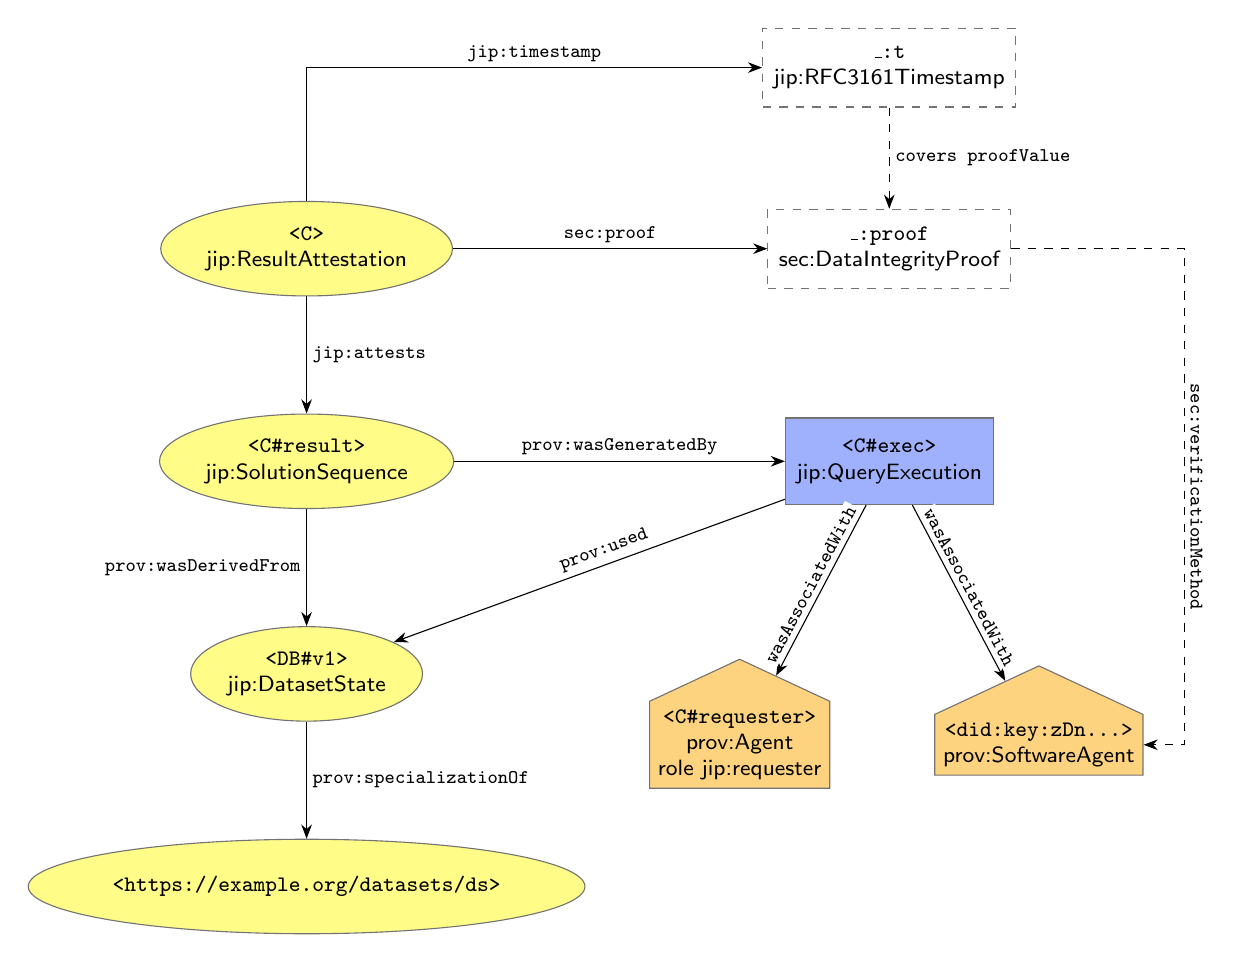
\begin{tikzpicture}[
  font=\sffamily\footnotesize, >={Stealth[length=1.8mm]},
  entity/.style={ellipse, draw=black!55, fill=provEntity, align=center, inner sep=1pt, minimum height=12mm},
  activity/.style={rectangle, draw=black!55, fill=provActivity, align=center, inner sep=4pt, minimum height=11mm},
  agent/.style={signal, signal to=north, signal pointer angle=130, draw=black!55, fill=provAgent, align=center, inner sep=3pt},
  plain/.style={rectangle, draw=black!55, dashed, fill=white, align=center, inner sep=4pt, minimum height=10mm},
  lbl/.style={font=\ttfamily\scriptsize, fill=white, inner sep=1pt},
]
\node[entity]   (cert)   at (0,0)      {\texttt{<C>}\\jip:ResultAttestation};
\node[plain]    (proof)  at (7.4,0)    {\texttt{\_:proof}\\sec:DataIntegrityProof};
\node[entity]   (result) at (0,-2.7)   {\texttt{<C\#result>}\\jip:SolutionSequence};
\node[activity] (exec)   at (7.4,-2.7) {\texttt{<C\#exec>}\\jip:QueryExecution};
\node[entity]   (state)  at (0,-5.4)   {\texttt{<DB\#v1>}\\jip:DatasetState};
\node[agent]    (agent)  at (9.3,-6.3) {\texttt{<did:key:zDn...>}\\prov:SoftwareAgent};
\node[entity]   (dset)   at (0,-8.1)   {\texttt{<https://example.org/datasets/ds>}};
\node[plain]    (stamp)  at (7.4,2.3)  {\texttt{\_:t}\\jip:RFC3161Timestamp};
\node[agent]    (user)   at (5.5,-6.3) {\texttt{<C\#requester>}\\prov:Agent\\role jip:requester};

\draw[->] (cert) -- node[lbl, above=1pt] {sec:proof} (proof);
\draw[->] (cert) |- node[lbl, above=1pt, pos=0.75] {jip:timestamp} (stamp);
\draw[->, dashed] (stamp) -- node[lbl, right=1pt] {covers proofValue} (proof);
\draw[->] (cert) -- node[lbl, right=1pt] {jip:attests} (result);
\draw[->] (result) -- node[lbl, above=1pt] {prov:wasGeneratedBy} (exec);
\draw[->] (exec) -- node[lbl, sloped, above=1pt] {wasAssociatedWith} (agent);
\draw[->] (result) -- node[lbl, left=1pt] {prov:wasDerivedFrom} (state);
\draw[->] (exec) -- node[lbl, sloped, above=1pt, pos=0.45] {prov:used} (state);
\draw[->] (state) -- node[lbl, right=1pt] {prov:specializationOf} (dset);
\draw[->, dashed] (proof.east) -- ++(2.2,0) |- node[lbl, sloped, above=1pt, pos=0.25] {sec:verificationMethod} (agent.east);
\draw[->] (exec) -- node[lbl, sloped, above=1pt] {wasAssociatedWith} (user);
\end{tikzpicture}
\caption{Structure of an attestation, drawn with the PROV conventions: entities as ellipses,
activities as rectangles, agents as pentagons; \code{wasAssociatedWith} is
\code{prov:wasAssociatedWith}. The dashed proof and timestamp nodes are not
part of PROV. The proof's verification method is the key in the agent's \code{did:key}; the
optional timestamp covers the proof's signature value. If the request was authenticated, the
execution is also associated with the requester, in the role \code{jip:requester} (a
\code{prov:qualifiedAssociation}).}
\label{fig:prov}
\end{figure}

\Needspace{10\baselineskip}
\begin{lstlisting}[language=Turtle, caption={An attestation from the demo, with prefixes added and long literals shortened.}, label={lst:attestation}]
PREFIX c:   <urn:uuid:cdd15485-9ab6-40a8-9993-7827c00606d3#>
PREFIX db:  <urn:uuid:69fd58e1-ed99-470f-b95f-426569c251ea#>
PREFIX key: <did:key:zDnaevMM9EKy1i19P8jPV7bhmE3Q4dYZRia1RtP6sEqYNL8oz#>

<urn:uuid:cdd15485-9ab6-40a8-9993-7827c00606d3>
    a jip:ResultAttestation, prov:Entity ;
    jip:attests c:result ;
    sec:proof [
        a sec:DataIntegrityProof ;
        sec:cryptosuite "ecdsa-rdfc-2019"^^sec:cryptosuiteString ;
        sec:verificationMethod key:zDnaevMM9EKy1i19P8jPV7bhmE3Q4dYZRia1RtP6sEqYNL8oz ;
        sec:proofPurpose sec:assertionMethod ;
        dcterms:created "2026-11-19T16:31:40Z"^^xsd:dateTime ;
        sec:proofValue "z2zG41vUXXhb...LFi2RNw9"^^sec:multibase ] ;
    jip:timestamp [
        a jip:RFC3161Timestamp ;
        jip:timestampToken "MIIXaQYJKoZIhvcNAQcCoIIXWjCC..."^^xsd:base64Binary ;
        jip:timestampAuthority <http://timestamp.digicert.com> ;
        jip:timestampTime "2026-11-19T16:31:41Z"^^xsd:dateTime ] .

c:result a jip:SolutionSequence, prov:Entity ;
    prov:wasGeneratedBy c:exec ;
    prov:wasDerivedFrom db:v1 ;
    jip:variable "email", "name" ;
    jip:ordered true ;
    jip:solutionCount 3 ;
    jip:canonicalization <https://www.w3.org/TR/rdf-canon/> ;
    jip:digestAlgorithm "SHA-256" ;
    jip:digest "feb2d70a55e34ba756145d9ff3960f09656a558890b08d68505be90ef06efebe" .

c:exec a jip:QueryExecution, prov:Activity ;
    prov:used db:v1 ;
    prov:wasAssociatedWith <did:key:zDnaevMM9EKy1i19P8jPV7bhmE3Q4dYZRia1RtP6sEqYNL8oz> ;
    prov:wasAssociatedWith c:requester ;
    prov:qualifiedAssociation [ a prov:Association ;
        prov:agent c:requester ; prov:hadRole jip:requester ] ;
    prov:startedAtTime "2026-11-19T16:31:40.939694267Z"^^xsd:dateTime ;
    prov:endedAtTime   "2026-11-19T16:31:40.959000657Z"^^xsd:dateTime ;
    jip:servicePattern "SELECT ?name ?email WHERE { ... } ORDER BY ?name" ;
    jip:queryText "PREFIX jip: <https://larsw.xyz/jip/> ..." .

db:v1 a jip:DatasetState, prov:Entity ;
    jip:dataVersion 1 ;
    prov:specializationOf <https://example.org/datasets/ds> .

<did:key:zDnaevMM9EKy1i19P8jPV7bhmE3Q4dYZRia1RtP6sEqYNL8oz>
    a prov:SoftwareAgent ;
    rdfs:label "jena-intrinsic-provenance 0.16.0 on Apache Jena 6.2.0" .

c:requester a prov:Agent ;
    jip:principal "alice" ;
    jip:authenticationScheme "BASIC" .
\end{lstlisting}

The attestation holds the digest of the rows and never the rows themselves, so its size
does not grow with the result. It does contain the query text, which has privacy implications
(Section~\ref{sec:risks}).

\subsection{The Requester}
\label{sec:requester}

An attestation can say who asked for it. If the HTTP request was authenticated, the query
execution is associated with a second agent besides the server's key. This agent,
\code{<C\#requester>}, is a \code{prov:Agent} with the authenticated name
(\code{jip:principal}) and, if known, the authentication scheme
(\code{jip:authenticationScheme}). A qualified association gives it the
role \code{jip:requester}, which separates it from the server agent. The statement is part of
the signed document, so the server vouches that it authenticated this principal; it says
nothing about how strong that authentication was. Anonymous requests have no requester.
Recording can be turned off with the setting \code{jip:recordRequester} or the environment
variable \code{PROVENANCE\_RECORD\_REQUESTER}. The verifier reports the requester (Example~\ref{lst:verify}).

The module takes the requester from the servlet request (\code{getRemoteUser()}), so it works
with whatever authenticated the request: Fuseki's Shiro module, its password file, or a
bearer-token filter. Fuseki does not pass the HTTP user into the query's context, but it
evaluates the query on the request's thread. A servlet filter therefore records the user per
thread, and the attest executor reads it there. The filter must run after the authentication filter.
Fuseki modules add filters in two steps, \code{prepare} and \code{configured}; authentication
modules use the first, so the module adds its filter in the second. Shiro does not report the
scheme through \code{getAuthType()}, so the filter falls back to the scheme of the
\code{Authorization} header. Embedded applications can put the requester into the query context
instead.

\subsection{Signing}
\label{sec:signing}

The signature follows \code{ecdsa-rdfc-2019} for P-256 and P-384 keys and
\code{eddsa-rdfc-2022} for Ed25519 keys, and is applied to the attestation graph directly.
Let $D$ be the attestation graph without the proof, and $P$ the proof options: the type of the
proof node, the cryptosuite, the creation time in whole seconds, the verification method, and
the proof purpose. With $\mathrm{C}$ for RDFC-1.0 canonicalization and $\Vert$ for
concatenation, the signer computes
\begin{align*}
  h &= H(\mathrm{C}(P)) \;\Vert\; H(\mathrm{C}(D)), \\
  \mathit{proofValue} &= \texttt{z} \;\Vert\; \mathrm{base58btc}(\mathrm{Sign}_{\mathit{sk}}(h)),
\end{align*}
where $H$ is SHA-256 for Ed25519 and P-256 keys and SHA-384 for P-384 keys, and
$\mathrm{Sign}$ is Ed25519, or ECDSA with $H$, which yields $r \Vert s$. The signer then adds
the proof options, the proof value, and the triple \code{<C> sec:proof \_:proof} to the
graph. A verifier removes the proof node's triples and the \code{sec:proof} link to
recover $D$, drops the proof value to recover $P$, and checks the signature with the public
key from the verification method. It also checks that the cryptosuite fits the key type, so
an ECDSA signature cannot pass as \code{eddsa-rdfc-2022} or the other way round.

In the JSON-LD form used by Verifiable Credentials, the proof sits in a separate named graph,
because the security context declares \code{sec:proof} with an \code{@graph} container. Here
the proof triples sit in the attestation graph, and the verifier separates them by structure.
The hash and signature computation is the cryptosuite's, unchanged. The proof options
canonicalize to the bytes in the specifications' test vectors, and the module reproduces or
verifies the vectors' proof values (Section~\ref{sec:conformance}). Off-the-shelf Verifiable
Credential verifiers nevertheless do not accept an attestation as it is, because they expect a
credential document in JSON-LD.

\subsection{Timestamps}
\label{sec:timestamps}

The times in an attestation come from the server's clock: \code{prov:startedAtTime},
\code{prov:endedAtTime}, and the proof's \code{dcterms:created}. They are only as trustworthy
as the server. Optionally, a time-stamping authority (Section~\ref{sec:tsp}) co-signs each
attestation. The message imprint is
\[
  \mathit{imprint} = \mathrm{SHA\text{-}256}(\mathrm{Sign}_{\mathit{sk}}(h)),
\]
the hash of the raw signature decoded from \code{sec:proofValue}. The signature covers the
whole attestation, so the token does too, and the Data Integrity proof itself is unchanged.
The request carries a random 64-bit nonce and asks for the TSA's certificate, so the token can
be checked offline. The executor accepts a reply only if it grants a token for the same
imprint and nonce and the token's signature verifies.

The token is added after signing, as a node of its own:
\Needspace{6\baselineskip}
\begin{lstlisting}[language=Turtle, numbers=none]
<C> jip:timestamp _:t .
_:t a jip:RFC3161Timestamp ;
    jip:timestampToken "MIIXaQYJKoZIhvcNAQcCoIIXWjCC..."^^xsd:base64Binary ;
    jip:timestampAuthority <http://timestamp.digicert.com> ;
    jip:timestampTime "2026-11-19T16:31:41Z"^^xsd:dateTime .
\end{lstlisting}
Only the token is evidence. The authority and the time are copies for queries over the
attestation store; the verifier reports what the token says. The timestamp triples are not part
of the signed document $D$: a verifier removes the \code{jip:timestamp} links and the triples
of the timestamp nodes before it checks the proof. Removing them cannot hide a change, because
removing any signed triple makes the proof fail.

The setting \code{jip:timestampAuthorities} lists TSA URLs in priority order. For each
attestation they are asked one at a time, each with its own timeout
(\code{jip:timestampTimeout}, 5~s by default), and the first valid token is used. A TSA that
fails is moved to the end of the list for 60~s, so a TSA that is down costs one timeout a
minute rather than one per attestation. It is still tried if all others fail.

A TSA request is a network round trip to a third party, typically a few hundred milliseconds,
and several timeouts if TSAs are down. By default (\code{jip:timestampMode async}) the query
does not wait for it. The executor stores the signed attestation and, in the same write
transaction, records it as pending with a triple
\code{<C> jip:timestampPendingSince "..."} in the store's graph
\code{jip:pendingTimestamps}. The query returns at once. A background thread fetches the token.
Then, in one transaction, it adds the timestamp triples to the attestation graph and removes
the pending triple. It does so only if the attestation is still pending, so an attestation
cannot receive two tokens. If no TSA answers, the thread tries again after 5, 15, and 30~s, after 1, 2, and
5~min, and then every 10~min. One thread per configuration fetches the tokens one after another,
because public TSAs limit request rates. Because the pending state is in the store, a restart
loses nothing: when Fuseki has started, the module queues the pending attestations again.

While an attestation is pending, its endpoint answers \code{202 Accepted} instead of the
attestation, with \code{Retry-After} set to the seconds until the next attempt and a short JSON
status (Example~\ref{lst:pending}). A client fetches the attestation again after that time and
gets it with its timestamp. Status 202 is more appropriate than 503: the server is healthy
and the attestation exists; only its processing is unfinished.

\Needspace{6\baselineskip}
\begin{lstlisting}[basicstyle=\ttfamily\footnotesize, caption={The attestation endpoint right after the attested query of the demo.}, label={lst:pending}]
HTTP/1.1 202 Accepted
Retry-After: 1
Content-Type: application/json

{"attestation":"urn:uuid:cdd15485-9ab6-40a8-9993-7827c00606d3","status":"timestamp-pending",
 "pendingSince":"2026-11-19T16:31:40.965237224Z","retryAfter":1}
\end{lstlisting}

The policy (\code{jip:timestampPolicy}) decides what happens when no TSA answers. With
\code{optional}, the default, retries stop after \code{jip:timestampMaxWait} (10~min by
default) and the attestation is released without a timestamp. With \code{required}, the
attestation stays pending and the retries continue, so the endpoint keeps answering 202 until a
TSA answers. In the synchronous mode (\code{jip:timestampMode sync}), the query waits for the
token instead; without one, \code{optional} issues the attestation as it is and
\code{required} refuses the attestation. Environment variables (\code{PROVENANCE\_TSA\_URLS}, \code{\_MODE},
\code{\_POLICY}, \code{\_TIMEOUT}, and \code{\_MAX\_WAIT}) override the settings. Without a TSA
list, attestations have no timestamp and are never pending.

The read-only SPARQL view of the attestation store (Section~\ref{sec:store}) is a plain TDB2
service. It therefore already shows a pending attestation, signed but without its timestamp.
The graph \code{jip:pendingTimestamps} lists the attestations that are still waiting for one.

The protocol and CMS handling come from Bouncy Castle~\cite{bouncycastle}, because the JDK has
no public API for either. Bouncy Castle also handles key encodings: PKCS\#8 and the PEM text
format for the local Ed25519 key, compressed curve points for P-256 and P-384 \code{did:key}s, and the self-signed
certificate of a key created on a PKCS\#11 token. Signing and verifying use the JDK.

\subsection{Keys}
\label{sec:keys}

Where the key lives is pluggable. A \emph{signer provider} opens the server's signer: a key
type, a public key, and an operation that signs the hash data $h$. Providers are found with
Java's \code{ServiceLoader} and chosen by name with \code{PROVENANCE\_SIGNER}. Two providers
are built in.

\begin{description}[style=nextline, leftmargin=1.5em, font=\normalfont\code]
\item[pkcs11 (default)] A P-256 or P-384 key on a PKCS\#11 token, used through SunPKCS11; the
  attestations use \code{ecdsa-rdfc-2019}. The settings name the PKCS\#11 module, the slot, the PIN
  (directly or from a file), and the key's label. With \code{PROVENANCE\_PKCS11\_GENERATE} set
  to a curve, the module creates the key pair on the token if it is missing. It also creates a
self-signed certificate, because SunPKCS11 only lists private keys that have one.
\item[local] An Ed25519 key in a PKCS\#8 PEM file, with \code{eddsa-rdfc-2022}. The path comes
  from \code{PROVENANCE\_SIGNING\_KEY} or \code{jip.signingKey}, and a
  key is generated on first start if the file does not exist.
\end{description}

Another mechanism, such as a cloud key service or a remote signing service, is one more
provider. The PKCS\#11 signer uses ECDSA because Java 21's SunPKCS11 has no EdDSA support.
EdDSA support in tokens also varies: SoftHSM2, for example, offers it only in builds that enable it,
and key generation fails in some of them~\cite{softhsm704}. P-256 is supported by practically
every token, and \code{ecdsa-rdfc-2019} is the W3C counterpart of \code{eddsa-rdfc-2022}.

In the Docker setup the token is in a process and a container of its own
(Figure~\ref{fig:separation}). The signer container runs SoftHSM2 behind \code{p11-kit server}
and has no network at all. The Fuseki container loads \code{p11-kit-client.so}, and the two
share only the volume that holds the socket. On first start the signer initializes its token,
and the module creates the P-256 key on it through the socket, so the key is generated inside
the token and never exported. For each attestation, the module sends $h$ and receives
$r \Vert s$. If the signer process restarts, the next signature fails, and the module reconnects
and tries again. SunPKCS11 cannot re-initialize a PKCS\#11 module it has already loaded. The
module therefore loads a fresh copy of \code{p11-kit-client.so} from a new path, which the system loader treats
as a separate library with a new connection. The p11-kit versions on both sides must match:
a version 0.26 client and a 0.25 server could not create keys, so both images use the same
Ubuntu release.

\begin{figure}[htb]
\centering
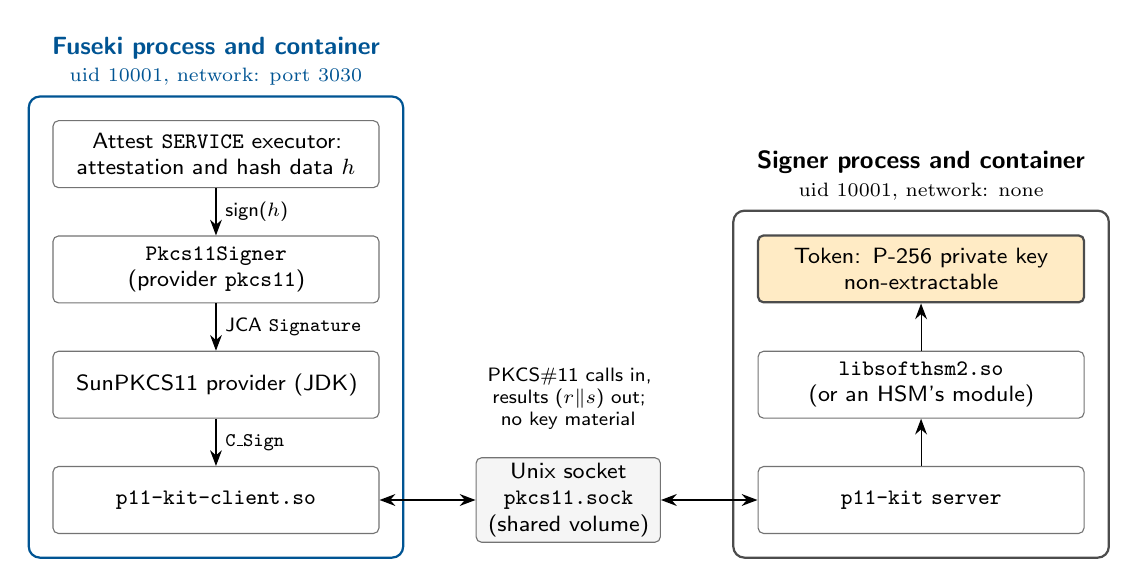
\begin{tikzpicture}[
  font=\sffamily\footnotesize, >={Stealth[length=2mm]},
  box/.style={draw=black!55, fill=white, rounded corners=2pt, align=center, text width=40mm,
              minimum height=8.5mm, inner sep=2pt},
  key/.style={draw=black!70, fill=provAgent!45, rounded corners=2pt, align=center, text width=40mm,
              minimum height=8.5mm, inner sep=2pt, thick},
  lbl/.style={font=\sffamily\scriptsize, fill=white, inner sep=1.2pt, align=center},
]
% Fuseki container
\node[box] (exec) {Attest \texttt{SERVICE} executor:\\attestation and hash data $h$};
\node[box, below=6mm of exec] (signer) {\texttt{Pkcs11Signer}\\(provider \texttt{pkcs11})};
\node[box, below=6mm of signer] (sun) {SunPKCS11 provider (JDK)};
\node[box, below=6mm of sun] (client) {\texttt{p11-kit-client.so}};
\node[draw=accent, thick, rounded corners=4pt, fit=(exec)(client), inner sep=3mm] (fc) {};
\node[font=\sffamily\small\bfseries, text=accent, anchor=south, align=center] at (fc.north)
  {Fuseki process and container\\[-1pt]\normalfont\scriptsize uid 10001, network: port 3030};

% Signer container: the server on the client's row, the token above it
\node[box, right=48mm of client] (server) {\texttt{p11-kit server}};
\node[box, above=6mm of server] (softhsm) {\texttt{libsofthsm2.so}\\(or an HSM's module)};
\node[key, above=6mm of softhsm] (token) {Token: P-256 private key\\non-extractable};
\node[draw=black!70, thick, rounded corners=4pt, fit=(token)(server), inner sep=3mm] (sc) {};
\node[font=\sffamily\small\bfseries, anchor=south, align=center] at (sc.north)
  {Signer process and container\\[-1pt]\normalfont\scriptsize uid 10001, network: none};

% The socket between them
\coordinate (mid) at ($(fc.east)!0.5!(sc.west)$);
\node[draw=black!55, fill=black!4, rounded corners=2pt, align=center, text width=22mm, inner sep=2pt]
  (sock) at (mid |- client) {Unix socket\\\texttt{pkcs11.sock}\\(shared volume)};

\draw[->] (exec) -- node[lbl, right=2pt] {sign($h$)} (signer);
\draw[->] (signer) -- node[lbl, right=2pt] {JCA \texttt{Signature}} (sun);
\draw[->] (sun) -- node[lbl, right=2pt] {\texttt{C\_Sign}} (client);
\draw[<->, thick] (client.east) -- (sock.west);
\draw[<->, thick] (sock.east) -- (server.west);
\draw[->] (server) -- (softhsm);
\draw[->] (softhsm) -- (token);
\node[lbl, text width=28mm, above=3mm of sock] {PKCS\#11 calls in,\\results ($r \Vert s$) out;\\no key material};
\end{tikzpicture}
\caption{Process separation of the PKCS\#11 signer in the Docker setup. The private key exists
only inside the token in the signer container, which has no network. Fuseki holds a handle and
the PIN and can ask for signatures, but it cannot read the key. In production, the signer
process loads an HSM's PKCS\#11 library instead of SoftHSM2.}
\label{fig:separation}
\end{figure}

Because a \code{did:key} contains its own public key, anyone can produce an attestation that
verifies against a key they generated themselves. A verifier must therefore compare the key with one it
already trusts, obtained through another channel. The verifier's \code{-{}-expect-key} option
does this comparison.

Keys are replaced from time to time, because a key has reached the end of its planned lifetime,
the token is replaced, or the key may have been exposed. Attestations signed before such a
\emph{rollover} must still verify afterwards, so the server publishes its old keys along with
the current one. The attestation store keeps a key history in the named graph
\code{jip:signingKeys}. It adds one triple \code{<did:key:...> jip:activatedAt t} each time the server
starts signing with a key that is not the latest one recorded. The module records the key when
the server starts and before the first attestation, so a restart with the same key writes
nothing. A rollover is a restart with another key, that is, another label on the token or another
key file; returning to an earlier key makes that key current again.

The endpoint \code{GET /\$/provenance/keys} publishes the history as a JSON Web Key Set
(JWK Set)~\cite{jwk}, with the media type \code{application/jwk-set+json}. The current key comes
first, then the retired keys, the most recently activated first. Each key has the standard
members for its type (\code{kty}, \code{crv}, \code{x}, and for EC keys \code{y}), \code{alg}
(\code{ES256}, \code{ES384}, or \code{EdDSA}), and \code{use} with the value \code{sig}. Its
\code{kid} is the verification method that the attestations name. Four further members describe
the key's place in the history: \code{did}, \code{status} (\code{current} or \code{retired}),
\code{activated} (the latest activation), and, for a retired key, \code{retired} (the time the
next key was activated). Example~\ref{lst:keys} shows the set after the demo's rollover.

\Needspace{22\baselineskip}
\begin{lstlisting}[basicstyle=\ttfamily\footnotesize, caption={The JWK Set returned by \code{GET /\$/provenance/keys} after the rollover in the demo (key identifiers shortened).}, label={lst:keys}]
{ "keys": [
  { "kty": "EC", "crv": "P-256",
    "x": "rMPSGsf0zd39WJGGiDOPpmhRl4mS9-54A4dxbnbW4SU",
    "y": "WWXnBpFL3dkRHd0_WZUvzvVBi6YFJL2OP1k9Uaa5gdA",
    "kid": "did:key:zDnaec...umfi#zDnaec...umfi",
    "alg": "ES256", "use": "sig",
    "did": "did:key:zDnaec...umfi",
    "status": "current",
    "activated": "2026-11-19T16:31:59.485371796Z" },
  { "kty": "EC", "crv": "P-256",
    "x": "vI-wOOeqFwu5gB9dhWDxc7BLRTMFZGTEyHXvV-I3oMk",
    "y": "1UhxV5CqvZu1X_EQxco98XZD3cIIRIeSvpXXQgQmTGE",
    "kid": "did:key:zDnaev...L8oz#zDnaev...L8oz",
    "alg": "ES256", "use": "sig",
    "did": "did:key:zDnaev...L8oz",
    "status": "retired",
    "activated": "2026-11-19T16:31:39.739495881Z",
    "retired": "2026-11-19T16:31:59.485371796Z" } ] }
\end{lstlisting}

The verifier's \code{-{}-trusted-keys} option reads such a set, saved through a channel the
verifier trusts, and accepts an attestation signed with any key in it. It derives each
\code{did:key} from the key material and ignores \code{kid}, so a set cannot vouch for a key it
does not contain. It does not check that an attestation was made while its key was current: the
proof's creation time is the server's own statement, and an asynchronous timestamp may land
after the rollover. A key that was retired because it was exposed should therefore be removed
from the trusted set instead of being kept as retired.

\subsection{Storing Attestations}
\label{sec:store}

Attestations go to a separate TDB2 database, as one named graph per attestation, named by the
attestation IRI. Writing them into the queried dataset would increment its version, so each
attestation would change the state it describes. The server-level setting
\code{jip:attestationStore} gives the location. The demo configuration exposes the store
read-only as \code{/provenance}, where the attestations can be queried as PROV-O. Each
attestation costs one write transaction on the store. The store is accessed through a small
interface, \code{AttestationStore}, so a file-based or remote store could replace it.

\subsection{Verification}
\label{sec:verification}

The verifier needs only the saved results and the attestation. Its checks are in a library,
\file{jip-verifier}, which depends on \code{jena-arq}, titanium-rdfc, and Bouncy Castle but not
on TDB2, Fuseki, or the signing key. Other Java programs can therefore verify attestations
themselves. A command, \longcode{xyz.larsw.jip.cli.Verify}, wraps the library; it is packaged as a
self-contained jar, and the Docker image runs it with the command \code{verify}. The
verification works in five steps:

\begin{enumerate}
\item Check the proof against the key in the \code{did:key}, over the attestation without its
  timestamps, with the cryptosuite that fits the key type. With \code{-{}-expect-key} or
  \code{-{}-trusted-keys}, also check that the key is one of the trusted keys.
\item Check each timestamp: the token's imprint must be the hash of the proof's signature, the
  TSA's signature must verify with the certificate in the token, and that certificate must be
  a time-stamping certificate valid at \code{genTime}. Then chain the TSA certificate, at
  \code{genTime} and without revocation checks, to trust anchors: the JVM's trust store
  (\code{-{}-tsa-trust system}, the default), the CA certificates in a PEM file, or none
  (\code{-{}-tsa-trust none}).
\item Select the rows that carry the attestation IRI. Their number must equal the
  attestation's \code{jip:solutionCount}. For an attestation with zero solutions, accept at most
  one row, and only if that row binds none of the attested variables.
\item Rebuild the \code{rs:} encoding from the attested variables, with \code{rs:index} only
  if the attestation says the result is ordered.
\item Canonicalize the encoding, hash it, and compare the digest with the attestation's.
\end{enumerate}

The verifier also reports the requester, if the attestation names one. The short options
\code{-r}, \code{-a}, and \code{-k} stand for \code{-{}-results}, \code{-{}-attestation}, and
\code{-{}-expect-key}. The option \code{-{}-expect-key} may be repeated, and \code{-{}-trusted-keys}
takes a JWK Set as published by the server. A broken timestamp makes the attestation invalid. An untrusted one is
reported, but it fails verification only with \code{-{}-require-timestamp}, which demands at
least one valid timestamp that is not untrusted. The verifier exits with
status 0 when everything matches, 1 when something does not, and 2 when the input
cannot be read. Example~\ref{lst:verify} shows a successful run, followed by a run on the same
results with one email address changed.

\Needspace{19\baselineskip}
\begin{lstlisting}[basicstyle=\ttfamily\footnotesize, caption={Verifier output for the demo results and for a tampered copy (key IRIs shortened, TSA line wrapped).}, label={lst:verify}]
$ verify -r results.srj -a attestation.ttl -k did:key:zDnaev...L8oz
Attestation     : urn:uuid:cdd15485-9ab6-40a8-9993-7827c00606d3
Signed by       : did:key:zDnaev...L8oz#zDnaev...L8oz
Signature       : OK
Timestamp       : OK  2026-11-19T16:31:41Z  (trusted)
  TSA           : C=US,O=DigiCert\, Inc.,CN=DigiCert SHA256 RSA4096 Timestamp
                  Responder 2026 1  via http://timestamp.digicert.com
Requested by    : alice (BASIC)
Dataset state   : urn:uuid:69fd58e1-ed99-470f-b95f-426569c251ea#v1  (version 1)
Solutions       : 3 attested, 3 row(s) carry this attestation
Result digest   : OK
VERIFIED

$ verify -r results-tampered.srj -a attestation.ttl -k did:key:zDnaev...L8oz
...
Result digest   : MISMATCH
Problem         : Result digest mismatch: attestation feb2d70a...f06efebe, rows b1c94dd9...92ecdc56
NOT VERIFIED
\end{lstlisting}

Because the verifier rebuilds the encoding from the delivered rows, the outer query must
return the attested variables unchanged. If the outer query renames, drops, or filters them,
the delivered rows no longer match the attestation. For an ordered attestation, the rows must
also arrive in the attested order.

% ====================================================================================
\section{Integration with Fuseki}
\label{sec:fuseki}

The module is loaded through two of Jena's plug-in mechanisms and changes nothing in Jena or
Fuseki (R6). Jena's subsystem loader finds \code{InitJIP}, a \code{JenaSubsystemLifecycle}, through the
Java \code{ServiceLoader}. It registers the assembler for \code{jip:VersionedDatasetTDB2}, the
two functions, and the service executor. Fuseki finds \code{ProvenanceFusekiModule}, a
\code{FusekiAutoModule}, the same way. It adds the servlet for \code{/\$/provenance/*}, the
header filter, and the requester filter (Section~\ref{sec:requester}), and logs the
\code{did:key} when the server starts. Putting the jar on Fuseki's
classpath is enough to load both. Example~\ref{lst:config} shows the relevant part of the
Fuseki configuration.

\Needspace{14\baselineskip}
\begin{lstlisting}[language=Turtle, caption={Fuseki configuration for the versioned dataset and the attestation store (excerpt of \textit{docker/config.ttl}).}, label={lst:config}]
[] a fuseki:Server ;
   ja:context [ ja:cxtName "https://larsw.xyz/jip/attestationStore" ;
                ja:cxtValue "/fuseki/databases/provenance" ] ;
   ja:context [ ja:cxtName "https://larsw.xyz/jip/maxSolutions" ;
                ja:cxtValue "10000" ] .

:dataset a jip:VersionedDatasetTDB2 ;          # instead of tdb2:DatasetTDB2
    tdb2:location "/fuseki/databases/ds" ;
    jip:datasetIRI <https://example.org/datasets/ds> .   # optional

:provDataset a tdb2:DatasetTDB2 ;              # attestation store, served read-only
    tdb2:location "/fuseki/databases/provenance" .
\end{lstlisting}

The signer is configured through the environment (Section~\ref{sec:keys}), and the timestamp
settings of Section~\ref{sec:timestamps} go into the same server context as the store. The
demo's \file{docker-compose.yml} sets them through the environment instead, with DigiCert,
Sectigo, and FreeTSA as the priority list, so the list can change without editing the
configuration file.

Table~\ref{tab:endpoints} lists the HTTP endpoints the module adds. The Docker image passes
its own Shiro configuration to Fuseki (\file{docker/shiro.ini}, replaceable with
\code{FUSEKI\_SHIRO}). It requires HTTP Basic authentication, with the demo users alice and
bob, for the dataset, the attestation store, and attestations, because attestations name their
requesters. The signing keys, the data versions, and the ping endpoint stay public, and the rest
of the administration area is limited to localhost.

\begin{table}[ht]
\centering
\caption{HTTP endpoints added by the module.}
\label{tab:endpoints}
\small
\begin{tabularx}{\linewidth}{@{}>{\raggedright\arraybackslash}p{62mm}>{\raggedright\arraybackslash}X@{}}
\toprule
Endpoint & Returns \\
\midrule
\code{GET /\$/provenance/attestation/\{uuid\}} & The attestation as Turtle, JSON-LD, N-Triples,
N-Quads, or RDF/XML, chosen by \code{Accept} or \code{?format=}. While its timestamp is
pending: \code{202 Accepted} with \code{Retry-After} (Example~\ref{lst:pending}). \\
\code{GET /\$/provenance/keys} & The current and retired signing keys as a JWK Set
(Example~\ref{lst:keys}). \\
\code{GET /\$/provenance/version/\{dataset\}} & The persistent and internal versions of a
dataset. \\
\bottomrule
\end{tabularx}
\end{table}

The Maven build has three modules: the verifier library, the verifier command, and the Fuseki
module. The Fuseki module's jar is the one Fuseki loads. Jena and Fuseki are \code{provided}
dependencies; the verifier library and titanium-rdfc are shaded in, the latter relocated.
Fuseki's server jar already contains Bouncy Castle's \code{bcprov}, unrelocated. The module
therefore shades in only \code{bcpkix} and \code{bcutil} at the same version (1.84) and links against
Fuseki's copy; none of their classes overlap with the server jar. These dependencies enlarge the
jar from 141~KB to about 1.9~MB. The verifier command is a separate jar that bundles Jena and
Bouncy Castle.

The Docker image is built in two stages. The first stage builds both jars in the
\longcode{maven:3.9-eclipse-temurin-21} image and runs the test suite on Java~21. It also
installs SoftHSM2, so that the PKCS\#11 tests run against a real token. The second stage starts
from \longcode{eclipse-temurin:21-jre-noble} and downloads \file{jena-fuseki-server-6.2.0.jar}
from Maven Central, checked against a pinned SHA-256 hash. The server runs as an unprivileged
user, with one volume for \file{/fuseki} and port 3030. The runtime image adds
\code{p11-kit-client.so} and points the PKCS\#11 signer at the signer's socket. A second image,
the signer, holds SoftHSM2 and \code{p11-kit server}; Docker Compose starts it first, without
network access, and shares its socket volume with Fuseki. The image's entry point also runs the
verifier, so that a client can check attestations with the same image without installing Java.

% ====================================================================================
\section{Evaluation}
\label{sec:eval}
% ###AQ: Add a lead-in sentence saying what Section 6 covers?

\subsection{Test Suite}
\label{sec:tests}

The build runs 171 tests, listed in Table~\ref{tab:tests}. They pass on Java 21 during the
Docker build and on OpenJDK 25 on the development machine. Where SoftHSM2 is not installed,
the four PKCS\#11 tests are skipped.

\begin{table}[htbp]
\centering
\caption{Test classes and what they cover.}
\label{tab:tests}
\footnotesize
\begin{tabularx}{\linewidth}{@{}>{\raggedright\arraybackslash}p{50mm}r>{\raggedright\arraybackslash}X@{}}
\toprule
Test class & Tests & Coverage \\
\midrule
\code{RdfCanonW3CTest} & 65 & The W3C RDFC-1.0 test suite, run through the Jena adapter. \\
\code{DataVersionTest} & 7 & Increment rules, snapshot versions under concurrent readers,
the functions, restart with stable identity, compaction, journal replay before open. \\
\code{ResultSetEncodingTest} & 7 & Row order with and without \code{rs:index}, value changes,
duplicates, blank nodes, empty results, rejection of RDF 1.2 terms. \\
\code{DataIntegrityProofTest} & 8 & The \code{eddsa-rdfc-2022} test vectors, tampering,
\code{did:key} encoding, base58 encoding. \\
\code{EcdsaDataIntegrityProofTest} & 14 & The \code{ecdsa-rdfc-2019} test vectors for P-256
and P-384: \code{did:key}s, hashes, canonical proof configuration, hash data, the vector
signature, signing with the vector key, and a cryptosuite that does not fit the key. \\
\code{SigningKeyTest} & 7 & The signing key against the test vectors, PEM round trip and
persistence, keys written by OpenSSL and the JDK, rejection of other key types and mismatched
public keys. \\
\code{KeyHistoryTest} & 3 & The key history in the attestation store across a rollover and a
return to an earlier key; the JWK Set's order, status, activation and retirement times,
\code{alg}, and \code{kid}; reading the set back as trusted keys; a forged \code{kid}. \\
\code{ProvenanceKeysTest} & 7 & Choosing the signer, error messages for a missing module or key
setting, PIN files, and the \code{did:key}, JWK, and PEM forms of P-256 and P-384 keys. \\
\code{Pkcs11SignerTest} & 4 & On a SoftHSM2 token: P-256 and P-384 keys created on the token,
signing, finding an existing key, a missing key, a whole attestation. \\
\code{AttestationTimestampsTest} & 6 & Timestamps against a test TSA: the proof stays valid,
trust anchors, a token for another signature, a corrupted token, TSA certificate validity at
\code{genTime}, reply and request matching. \\
\code{TimestampAuthoritiesTest} & 4 & Fallback through a refusing and an unreachable TSA,
cooldown order, configuration parsing. \\
\code{AttestServiceTest} & 22 & Round trips for ordered and unordered results, tampering,
both empty-result modes, variable names, the cap, unversioned datasets and \code{SILENT}, the
write-transaction refusal, versions after updates, correlated calls, timestamped
attestations, both timestamp policies in both modes, a query that does not wait for a held-back
TSA, resuming pending timestamps after a restart without a second token, the requester from
the query context and from the request thread, signed and verified, turned off, and absent for
anonymous requests, a set of trusted keys, and the key history. \\
\code{CanonicalizationCapacityTest} & 1 & Digest time at 10,000 solutions. \\
\code{FusekiIntegrationTest} & 2 & End to end over HTTP with \file{docker/config.ttl}; 202
with \code{Retry-After} while a timestamp is pending, then 200; the JWK Set at
\code{/keys}. \\
\code{AuthenticatedRequesterTest} & 1 & Over HTTP with Basic authentication (Fuseki's password
file): 401 without a login; alice's and bob's attestations name them and verify. \\
\code{VocabularyTest} & 3 & \file{vocab/jip.ttl} defines every \code{jip:} term the code uses,
and no others (Appendix~\ref{app:vocab}). \\
\code{VerifyTest} & 10 & Exit status of the verifier command for good, bad, and missing
arguments, including the timestamp options and the trusted-key set. \\
\midrule
Total & 171 & \\
\bottomrule
\end{tabularx}
\end{table}

\subsection{Conformance}
\label{sec:conformance}

The W3C test suite for RDFC-1.0~\cite{rdfcsuite} is included in the repository with its
license and source commit. All 65 tests pass. They include the tests that check the blank node
mapping, the variants that use SHA-384, the tests for N-Quads escaping, and the negative test
with a poison graph. The negative test has to fail within a time limit, here 3~s.

For the signature, the module reproduces the test vectors of the Data Integrity EdDSA
specification~\cite{eddsa}: the key identifiers, the two SHA-256 hashes, the canonical proof
configuration, and the proof value, each byte for byte. For the ECDSA
specification~\cite{ecdsa}, it matches the P-256 and P-384 vectors for the \code{did:key}s, the
hashes, the canonical proof configuration, and the hash data. ECDSA signatures are randomized,
so the vector's signature is verified rather than reproduced, and signing is checked by signing
with the vector's key and verifying the result.

\subsection{End-to-End Demo}
\label{sec:demo}

The script \file{scripts/demo.sh} runs against the Docker image. Table~\ref{tab:demo} shows a
run that started with empty volumes, with the PKCS\#11 signer in its own container, HTTP Basic
authentication, and the default TSA list: DigiCert, Sectigo, and FreeTSA. The step numbers are
those the script prints.

\begin{table}[htbp]
\centering
\caption{Observations from one run of the demo script.}
\label{tab:demo}
\small
\begin{tabularx}{\linewidth}{@{}r>{\raggedright\arraybackslash}p{52mm}>{\raggedright\arraybackslash}X@{}}
\toprule
No. & Step & Observation \\
\midrule
1 & Start the signer and Fuseki & The module creates a P-256 key on the signer's token;
\code{/\$/provenance/keys} lists it, \code{ES256}, as the current key
\code{did:key:zDnaev...L8oz}. \\
2 & Load three people through the Graph Store Protocol & Response header
\code{X-Dataset-Version: 1}. \\
3 & Run the attested query (Example~\ref{lst:query}), first without logging in, then as
alice & Without a login: HTTP 401. As alice: three rows with one attestation;
\code{X-Dataset-Version: 1}. \\
4 & Fetch the attestation right after the query & \code{202 Accepted},
\code{Retry-After: 1}, status \code{timestamp-pending} (Example~\ref{lst:pending}); about a
second later 200 with the timestamped attestation. \\
5 & Verify in a separate container & \code{VERIFIED}, exit status 0; the P-256 signature
from the token checks out; requested by alice (\code{BASIC}). Timestamp from
DigiCert, trusted through the JVM trust store, one second after the proof's creation
time. \\
6 & Change one email address and verify & Digest mismatch, exit status 1. \\
7 & As bob, insert a fourth person and query again & Update header 2; new attestation for 4
solutions at version 2, requested by bob, verified. \\
8 & Attest a pattern with no match & One row with only \code{?attestation}; attestation with 0
solutions, verified. \\
9 & Compare the counters & Persistent 2, internal 2. \\
10 & Restart the container, then insert one more person & After the restart: persistent 2,
internal 0. After the insert: persistent 3, internal 1. \\
11 & Query the attestation store & Three attestations, at versions 1, 2, and 2, requested by
alice, bob, and alice, each timestamped by DigiCert. \\
12 & Put an unreachable TSA first in the list, query again & The server logs the failed TSA
and falls back to DigiCert; the new attestation at version 3 verifies. \\
13 & Restart the signer container, query again & The first signature fails, the module
reconnects with a fresh copy of \code{p11-kit-client.so}, and the new attestation, signed with
the same key, verifies. \\
14 & Restart Fuseki with another key label (key rollover), query again & The module creates a
second P-256 key; \code{/keys} lists it as current and the first as retired
(Example~\ref{lst:keys}). With \code{-{}-trusted-keys} and that set, the new attestation and
the step-3 attestation both verify. \\
\bottomrule
\end{tabularx}
\end{table}

\subsection{Performance}
\label{sec:perf}

Apart from evaluating the query, the only step of attestation whose cost grows with the
number of solutions is the digest. The capacity test digests 10,000 solutions of two variables
after a warm-up run on 100 solutions. Table~\ref{tab:perf} shows three consecutive runs, each
in a fresh JVM, of version 0.15.0 on a lightly loaded desktop with an Intel Core Ultra~7 265
and OpenJDK 25.0.4.1. The digest runs on one thread.

\begin{table}[ht]
\centering
\caption{Time to encode, canonicalize, and hash 10,000 solutions with two variables (three runs).}
\label{tab:perf}
\small
\begin{tabular}{@{}lr@{}}
\toprule
Result & Time (ms) \\
\midrule
Unordered, all rows distinct & 359--375 \\
Ordered, all rows distinct & 221--235 \\
Unordered, 10 distinct rows repeated 1,000 times & 277--283 \\
\bottomrule
\end{tabular}
\end{table}

The ordered case is the fastest because of how RDFC-1.0 assigns labels
(Section~\ref{sec:rdfc}). In an unordered encoding, every solution node is linked to the result
node and to its own binding nodes, all blank. All 10,000 solution nodes therefore have the same
first-degree hash, and each one needs the N-degree step. In an ordered encoding, \code{rs:index}
gives each solution node a unique first-degree hash, and that step is skipped. All three cases
stay well below the limit of 10~s, which leaves room for wider rows. Solutions are held in
memory up to the cap, and the attestation store adds one write transaction per attestation.

% ====================================================================================
\section{Discussion}
\label{sec:discussion}
% ###AQ: Add a lead-in sentence saying what Section 7 covers?

\subsection{What an Attestation Proves}
\label{sec:trust}

A valid attestation, checked against a trusted key, shows that the holder of that key stated
that these rows were the solutions of this pattern against a given database state at a given
time. It does not show that the server evaluated the query correctly or that the data are true.
If the attestation names a requester, the server also states that it authenticated that user
for this query; the statement is only as good as the server's authentication. Without a
trusted key, a valid attestation shows only that the rows and the attestation belong together
(Section~\ref{sec:keys}).

A compromised server can sign anything while it is compromised. With the PKCS\#11 signer,
however, it cannot take the key away. The key stays on the token, so the attacker's access ends
when the server is cleaned up, and an HSM can log or limit what is signed. The times inside the
attestation come from the server's clock. With a timestamp from a TSA that the verifier trusts,
the attestation is also known to have existed no later than the token's \code{genTime},
independently of that clock. The token says nothing about the times the server wrote.

\subsection{Reproducing an Attested Result}
\label{sec:reproduce}

An attestation names the database state it was computed from, but TDB2 keeps only the latest
state. Running the query again later gives a result for a later version, which will not match the
digest if the data have changed in between. Re-evaluating an attested query against its
original state requires a copy of the database taken at that version, for example a backup
whose name includes the database ID and version.

\subsection{Risks and Limitations}
\label{sec:risks}
% ###AQ: The list follows the heading directly; add a sentence that introduces it?

\begin{itemize}
\item Anyone who can run a query can create attestations, and each attestation is a write
  transaction on the attestation store. That can be used to flood the server with writes. Authentication or rate limiting is needed before real use.
\item Every attestation contains the full query text and, for authenticated requests, the
  user's name, so whoever can read the attestation store or fetch attestations sees who asked
  what. The demo requires a login for both; \code{jip:recordRequester} stops recording users.
  The demo's users and passwords are in plain text in \file{docker/shiro.ini}.
\item Tools such as \code{tdb2.tdbloader} that write to the database from another JVM
  without the module do not advance the version. A byte-for-byte copy of the database
  directory shares the original's database ID; if both copies receive writes, the pair of ID
  and version is no longer unique.
\item Each timestamped attestation costs one outgoing HTTP request, and public TSAs limit
  request rates. The requests run one at a time in the background, so a burst of attestations
  queues up and stays pending for longer. Production use needs a dedicated or contracted TSA.
  TSA certificates are not checked for revocation, and a timestamp is only as trustworthy as
  the TSA's key.
\item The PKCS\#11 PIN is in the Fuseki process. The key cannot be read, but whoever controls
  that process can have the token sign. SoftHSM2 stores its keys in files and only stands in
  for an HSM, and p11-kit's client/server forwarding is Linux-only.
\item Refused attestations reach the client as HTTP 500 instead of a 4xx status.
\item In embedded use with Jena 6.2.0, queries over TDB2 have to run inside a transaction,
  because lazily evaluated patterns fail outside one. This happens without the module too,
  and Fuseki always opens a transaction.
\item Jena's IRI checker warns about the \code{\#} in \code{did:key} verification method
  IRIs, which DID URL syntax allows. The verifier suppresses the warning when it reads an
  attestation.
\end{itemize}

\subsection{Future Work}
\label{sec:future}

Most of the complexity in Section~\ref{sec:recovery} exists because a component cannot join
TDB2 before journal recovery when the database is built from a Fuseki configuration file. A
hook in DBOE for registering components before recovery would remove the need for the custom
assembler and for the pre-open journal scan. A persistent \code{dataVersion} in TDB2 itself
would remove the component entirely.

Other extensions follow from the limitations above: packaging attestations as Verifiable
Credentials in JSON-LD so that existing verifiers accept them, access control and rate limits
for attestation, and HTTP status codes in the 4xx range for refused attestations. The verifier
could enforce key retirement by accepting a retired key only for attestations whose trusted
RFC~3161 time precedes the retirement. The key history could also record why a key was
retired, so that an exposed key is distrusted outright. Results larger than the cap would need an encoding that can be hashed while
streaming, for example a hash tree over chunks of rows, instead of holding all solutions in
memory. Timestamps could be batched, with one token over a hash tree of many attestations, to
reduce the number of TSA requests. Revocation data for TSA certificates could be collected
when the token is issued, so that a timestamp stays verifiable after the TSA certificate
expires. Ed25519 keys could move to PKCS\#11 once SunPKCS11 supports EdDSA, or through Java's
foreign function interface. Further signer providers could reach a cloud key service. A signer
that checks what it is asked to sign, for example by rate or by key usage, would limit
what a compromised server can do with the key.

% ====================================================================================
\section{Conclusion}
\label{sec:conclusion}

Both research questions have a positive answer, with conditions. TDB2's internal
\code{dataVersion} has the right increment rules but lives only in memory. A DBOE component
that writes its own REDO record makes the version persistent and atomic with the data. The
dataset must be declared as \code{jip:VersionedDatasetTDB2} so that the version can be
recovered before TDB2 opens the database. A \code{SERVICE} with a reserved IRI can attest the
solutions of any pattern. The solutions are encoded as RDF, canonicalized with RDFC-1.0,
hashed, and recorded in a PROV-O attestation that also names the authenticated user. The
attestation is signed with \code{ecdsa-rdfc-2019} by a key that stays on a PKCS\#11 token in a separate
process, or with \code{eddsa-rdfc-2022} and a local key. The attestation can be checked
offline, the cryptography agrees with the W3C test vectors, and 10,000 solutions take less
than 0.4~s to digest. An optional RFC~3161 timestamp over the signature adds evidence,
independent of the server, of when an attestation existed. Because the timestamp is fetched in
the background, it does not slow down the query.

An attestation shows what the key holder stated, not that the query was evaluated correctly
(Section~\ref{sec:trust}). Before production use, the module needs rate limits for attestation,
4xx status codes for refused attestations, and, for results above the cap, an encoding that can
be hashed while streaming (Sections~\ref{sec:risks} and~\ref{sec:future}).

% ====================================================================================
% Keep floats from drifting into the appendices or the bibliography.
\FloatBarrier
\appendix

\clearpage
\section{Reproducing the Results}
\label{app:reproduce}

The repository at \url{https://github.com/larsw/jip} contains everything needed to repeat the
measurements in this report. The commands below assume Docker with Compose v2, \code{curl}, and
\code{jq} for the demo, and Maven with Java 21 or later for the local build. The demo logs in as
the demo users of \file{docker/shiro.ini}; \code{JIP\_PORT} selects another host port if 3030 is
taken.

\Needspace{7\baselineskip}
\begin{lstlisting}[language=bash, caption={Commands to build, test, and run the demo.}, label={lst:reproduce}]
docker compose up -d --build    # build the module, run the tests on Java 21, start Fuseki
scripts/demo.sh --reset         # end-to-end demo; --reset deletes the demo volumes
mvn test                        # the 171 tests (PKCS#11 tests need SoftHSM2)
scripts/build-whitepaper.sh     # this report
\end{lstlisting}

\clearpage
\section{Vocabulary}
\label{app:vocab}

Table~\ref{tab:vocab} lists the terms of the \code{jip:} namespace. The file
\file{vocab/jip.ttl} in the repository defines them in RDFS and OWL, with labels, comments,
domains, and ranges. It places the attestation classes under PROV-O:
\code{jip:QueryExecution} is a subclass of \code{prov:Activity}, and the other three
attestation classes are subclasses of \code{prov:Entity}. The timestamp class
\code{jip:RFC3161Timestamp} is not a PROV class, and \code{jip:requester} is a \code{prov:Role}. The two functions are typed
as \code{sd:Function} from SPARQL 1.1 Service Description~\cite{sparqlsd}, and
\code{jip:VersionedDatasetTDB2} as a subclass of \code{ja:RDFDataset}. The file also describes \code{jip:dataVersionComponent}, a
context symbol the module uses internally. The test \code{VocabularyTest} fails if the file and
the code disagree about which terms exist.

The namespace is a slash namespace, so every term has an IRI of its own. A GitHub Actions
workflow publishes the file with GitHub Pages. The namespace IRI
\mbox{\url{https://larsw.xyz/jip/}} serves a page that describes all terms, and each term IRI, such as
\mbox{\url{https://larsw.xyz/jip/ResultAttestation}}, serves a page for that term. GitHub Pages
cannot negotiate content types, so these pages are HTML. Each embeds its RDF as JSON-LD and links
to Turtle, JSON-LD, and N-Triples versions of the vocabulary with \code{<link rel="alternate">}
elements.

\begin{table}[ht]
\centering
\caption{Terms in the \code{jip:} namespace.}
\label{tab:vocab}
\small
\begin{tabularx}{\linewidth}{@{}>{\raggedright\arraybackslash}p{44mm}>{\raggedright\arraybackslash}X@{}}
\toprule
Term & Meaning \\
\midrule
\code{jip:VersionedDatasetTDB2} & Assembler type for a TDB2 dataset with a persistent
version. \\
\code{jip:datasetIRI} & Configuration: the logical dataset that each dataset state
specializes. \\
\code{jip:attestationStore} & Server setting: location of the attestation database. \\
\code{jip:maxSolutions} & Server setting: largest result an attest call accepts. \\
\code{jip:timestampAuthorities} & Server setting: TSA URLs in priority order. \\
\code{jip:timestampPolicy} & Server setting: \code{optional} or \code{required}. \\
\code{jip:timestampTimeout} & Server setting: time allowed per TSA, in milliseconds. \\
\code{jip:timestampMode} & Server setting: \code{async} or \code{sync}. \\
\code{jip:timestampMaxWait} & Server setting: how long an optional timestamp is retried, in
milliseconds. \\
\code{jip:recordRequester} & Server setting: whether attestations name the authenticated user. \\
\code{jip:requestUser} & Query context: the requester, for embedded use. \\
\code{jip:dataVersion()} & Function: persistent version of the current snapshot. \\
\code{jip:tdbDataVersion()} & Function: TDB2's internal counter. \\
\midrule
\code{jip:ResultAttestation} & Class of attestations. \\
\code{jip:SolutionSequence} & Class of attested solution sequences. \\
\code{jip:QueryExecution} & Class of query executions. \\
\code{jip:DatasetState} & Class of dataset states. \\
\code{jip:attests} & Links an attestation to its solution sequence. \\
\code{jip:variable} & An attested variable name. \\
\code{jip:ordered} & Whether row order is part of the digest. \\
\code{jip:solutionCount} & Number of attested solutions. \\
\code{jip:canonicalization} & Canonicalization algorithm (RDFC-1.0). \\
\code{jip:digestAlgorithm}, \code{jip:digest} & Hash function and hexadecimal digest. \\
\code{jip:servicePattern}, \code{jip:queryText} & The inner pattern and the whole query as
SPARQL text. \\
\code{jip:dataVersion} & Version number of a dataset state. \\
\midrule
\code{jip:RFC3161Timestamp} & Class of timestamps over an attestation's signature. \\
\code{jip:timestamp} & Links an attestation to a timestamp. \\
\code{jip:timestampToken} & The time-stamp token in DER encoding, as base64. \\
\code{jip:timestampAuthority}, \code{jip:timestampTime} & Copies of the issuing TSA and its time,
for queries. \\
\code{jip:pendingTimestamps} & Graph in the attestation store listing pending attestations. \\
\code{jip:timestampPendingSince} & When an attestation started waiting for its timestamp. \\
\code{jip:signingKeys} & Graph in the attestation store holding the key history. \\
\code{jip:activatedAt} & When a key became the signing key. \\
\midrule
\code{jip:requester} & The requester's role (a \code{prov:Role}) in the query execution. \\
\code{jip:principal}, \code{jip:authenticationScheme} & The requester's authenticated name and how
it was authenticated. \\
\bottomrule
\end{tabularx}
\end{table}

\clearpage
% bibintoc sets no anchor; without one, the Contents entry links to the previous float.
\phantomsection
\printbibliography[heading=bibintoc]

\end{document}
